\chapter{Schleifenschlüsse und Graph-Optimierung}
\label{chapter:loop_closure}

Dieses Kapitel beschäftigt sich mit der Detektion von Schleifenschlüssen und der damit verbundenen Optimierung der initialen Schätzung einer Trajektorie beziehungsweise eines Pose-Graphen, entlang dessen ein Sensorsystem bewegt wurde. Im Folgenden wird zunächst näher auf den Detektionsschritt eingegangen. Auf Basis dessen wird in den drauf folgenden Abschnitten die in dieser Arbeit verwendete Methode zur Optimierung des Pose-Graphen eruiert.

\section{Detektion von Schleifenschlüssen}

Dieser Abschnitt befasst sich mit der Detektion von Schleifenschlüssen in einem Pose-Graphen. Die hier vorgestellte Methode kann sowohl in einem inkrementell erweiterten Pose-Grahen, zum Beispiel als zusätzlicher Schritt in einem SLAM Verfahren, als auch in einem Nachbearbeitungsschritt auf einen bereits fertigen Graphen angewandt werden. Die Methode und die Optimierung des Graphen ist dabei zunächst vollständig losgelöst von der TSDF-Karte, die im Anschluss optimiert wird. Mehr dazu in Kapitel \ref{chapter:map_update}. Die vorliegenden initiale Schätzung der Roboter-Trajektorie kann das Ergebnis eines inkrementellen SLAM Ansatzes sein oder lediglich auf Odometrie-Schätzung beruhen.

Bevor nach Schleifenschlüssen gesucht werden kann, gilt es zu bestimmen, von welcher Pose aus gesucht werden soll. In einem inkrementellen SLAM Verfahren wäre das jeweils die aktuell betrachtete, zuletzt in den Graphen eingefügte Pose. In einem Nachbearbeitungsschritt wird dieser inkrementelle Prozess imitiert, indem der Pose-Graph, beginnend von der ersten eingefügten Pose, abgelaufen wird. In beiden Fällen wird also ein Schleifenschluss mit Posen gesucht, die früher in den Graphen eingefügt wurden als die aktuelle Pose $P_{cur}$. In einem ersten Schritt wird hierzu eine Menge von Schleifenschluss-Kandidaten erstellt. Diese Menge ergibt sich aus der in \cite{borrmann2008globally, shan2020lio} vorgestellten euklidischen Distanzmetrik, die in dieser Arbeit verwendet wird. Eine Pose $P_i$ gilt als Schleifenschluss-Kandidat zu $P_{cur}$, wenn die euklidische Distanz zwischen den beiden Posen geringer ist als eine parametrisierbare Schwelle $d_{max}$. Zusätzlich zu diesem Parameter wird an dieser Stelle ein weiterer Parameter $d_{trav}$ eingeführt der die minimale Distanz definiert, die der Sensorsystem entlang des Teilpfades gegeben durch $P_i$ und $P_{cur}$ zurückgelegt hat. Um Posen zu identifizieren, die diese Voraussetzungen Erfüllen, wird ein \emph{k-d tree (k-d Baum)} \cite{bentley1975multidimensional} verwendet. Ein k-d Baum ist eine Datenstruktur zur Speicherung von (räumlichen) Informationen, die durch assoziative Suchen abgefragt werden können. Ein k-d Baum eignet sich aufgrund der optimierten Laufzeit besonders für räumliche Suchen. Dabei steht das \emph{k} für die Dimensionalität des Suchraums \cite{bentley1975multidimensional}. An dieser Stelle wird der k-d Baum zur Speicherung von \emph{3-d} Daten genutzt. Diese ergeben sich aus den Posen des Pfades. Vor jeder Detektion wird ein neuer k-d Baum aus den Translationsanteilen aller zuvor eingefügten Posen aufgebaut. Im Anschluss wird eine Radius-Suche durchgeführt, die alle Daten des k-d Baumes (hier 3-d Punkte) zurückliefert, deren euklidische Distanz zu einer übergebenen Position geringer ist als eine übergebene Schwelle. Die übergebene Position ist dabei der Translationsanteil von $P_cur$ und die übergebene Schwelle $d_max$. Ergebnis ist eine Menge von Kandidaten für Schleifenschlüsse $\mathbb{K} = \left\lbrace K_0, ..., K_k \right\rbrace$. Diese Arbeit verwendet die k-d Baum Implementation der \emph{Pointcloud Library (PCL)} \cite{rusu20113d}.

Über die generierten Kandidaten ist an dieser Stelle lediglich bekannt, dass sie sich im nicht optimierten Pfad in der Nähe der aktuellen Pose $P_{cur}$ befinden. Diese räumliche Nähe ist an dieser Stelle allerdings nur eine Annahme, die es zu verifizieren gilt. Als Basis für die Verifikation dient die in diesem Ansatz gegebene Datenbasis in Form von zu jeder Pose des Pose-Graphen $\mathfrak{P}_{init} = \left\lbrace P_0, ..., _n \right\rbrace$ zugehörigen Punktwolken $ \mathbb{C} = \left\lbrace C_0, ..., C_n \right\rbrace$. Für die aktuell betrachte Pose $P_{cur}$ und die zugehörige Punktwolke wird ein Scan-Matching gegen jeden Kandidaten aus  $\mathbb{K}$ und dessen zugehörigen Punktwolken $C_i$ durchgeführt und evaluiert. Konvergiert das Scan-Matching mit einer festgelegten Genauigkeit ist der Kandidat validiert. Im Folgenden wird die Punktwolke der aktuell betrachteten Pose $P_{cur}$ als Scan-Punktwolke $C_{scan}$ und die zum zu validierenden Kandidaten zugehörige Punktwolke als Model-Punktwolke $C_{model}$ bezeichnet. Grundlage für das Scan-Matching der beiden Punktwolken ist ein Algorithmus wie \emph{ICP}, \emph{GICP} oder vergleichbare Algorithmen zur Registrierung von Punktwolken. Diese Algorithmen liefern neben einer Information zur Konvergenz in der Regel zusätzlich ein Maß dafür zurück, wie gut die Punktwolken nach der Registrierung aufeinander passen. In dieser Arbeit werden hierzu die Implementationen der Algorithmen der Pointcloud Library \cite{rusu20113d} verwendet. Diese liefern für beide Algorithmen einen \emph{Fitness-Score ($\Gamma$)} zurück, der die durchschnittliche quadrierte Distanz zwischen einem Punkt der Scan-Punktwolke und dem euklidisch nächste Punkt der Model-Punktwolke nach Registrierung der Scan-Punktwolke an die Model-Punktwolke beschreibt. Nachfolgende Formel zeigt diesen Sachverhalt mit $s_i$ als aktuellen Scanpunkt und $m_i$ als zugehörigen, euklidisch nächsten Punkt der Model-Punktwolke und $N$ als Anzahl der Punkte in der Scan-Punktwolke.

\begin{myequation}
\Gamma = \frac{\sum_{i = 0}^{N} \norm{\vec{m_i} - \vec{s_i}}^2}{N}
\end{myequation}

Liegt der Fitness-Score unter eine vordefinierten Schwelle $\Gamma_{max}$, ist der Kandidat validiert.
Zusätzlich liefern die Algorithmen die bestimmte finale Transformation $T_{fin}$ der Registrierung von Scan zu Model. Da GICP und ICP deutlich bessere Ergebnisse erzielen, wenn zwischen den Daten bereits eine Initialschätzung vorliegt, wird eine solche, auf Basis der jeweiligen Pose-Differenzen, genutzt. Die Punktwolkendaten liegen hier jeweils relativ zur Pose, von derer sie aufgenommen wurden, vor. Für die Initialschätzung wird nun die Model-Punktwolke ins Koordinatensystem der Scan-Punktwolke transformiert. Dazu wird zunächst die Transformation $T_{model \rightarrow scan}$ über die zugehörigen Posen $P_{model}$ und $P_{scan}$ und die zugehörigen Transformationen $T_{model \rightarrow map}$ und $T_{scan \rightarrow map}$ von den Posen ins Ursprungskoordinatensystem bestimmt:

\begin{myequation}
T_{model \rightarrow scan} = T_{scan \rightarrow map}^{-1} \cdot T_{model \rightarrow map}
\end{myequation}

Im Anschluss wird jeder Punkt $p_{model}^i$ der Punktwolke $C_{model}$ mit der bestimmten Transformation $T_{model \rightarrow scan}$ transformiert. Nun ist die Model-Punktwolke in das Koordinatensystem der Scan-Punktwolke, gegeben die aktuellen Pose-Schätzungen, vortransformiert. Diese Vortransformation muss nach der anschließenden Registrierung mittels ICP, GICP oder einem ähnlichen Verfahren für die Berechnung der finalen Transformation berücksichtigt werden. Dies ist in Abbildung \ref{fig:LoopIdentifikation} dargestellt. Sie führt zusätzlich die vom zur Registrierung berechneten Algorithmus bestimmte Transformation $T_{reg}$, sowie die sich daraus ergebene neue, approximative Pose $P_{scan}'$, von der die Scan-Punktwolke aufgenommen wurde. Die finale Transformation $T_{scan' \rightarrow model}$ die im weiteren Verlauf für die Optimierung des Pose-Graphen benötigt wird ergibt sich wie folgt:

\begin{myequation}
\label{math:final_transformation}
T_{scan' \rightarrow model} = T_{model \rightarrow scan}^{-1} \cdot T_{reg}
\end{myequation}

\begin{figure}
		\centering
		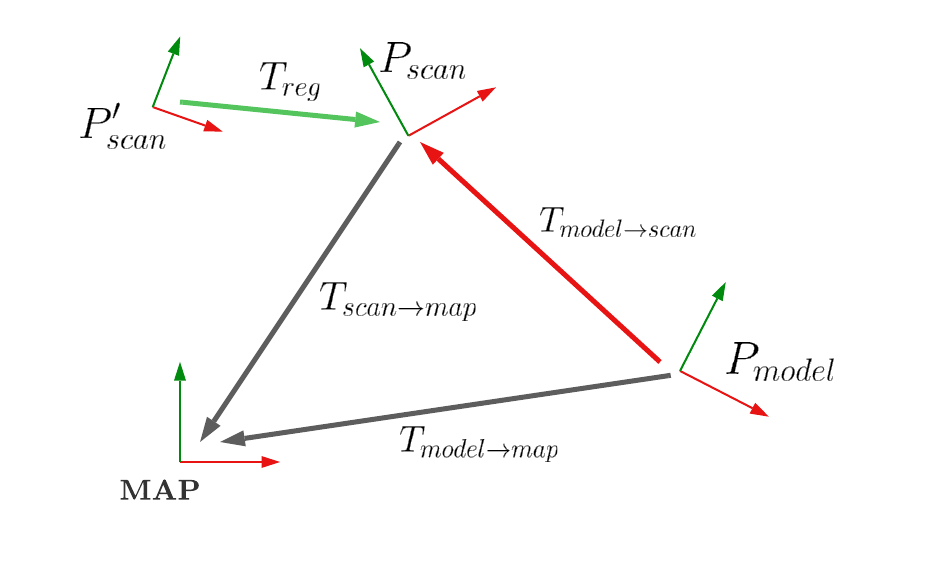
\includegraphics
			[scale=0.3]
			{LoopIdentifikation}
		\caption
			[Caption for LOF]{Diese Grafik stellt die Posen und Transformationen dar, die bei der Detektion eines Schleifenschlusses zur Verwendung kommen. Dabei bestimmt $T_{model \rightarrow scan}$ die Vortransformation vom lokalen Model-Koordinatensystem in das des Scans (dargestellt in rot). In grün dargestellt ist die Transformation $T_reg$, die von dem verwendeten Algorithmus zur Registrierung der Scan-Punktwolke an die mit $T_{model \rightarrow scan}$ vortransformierte Model-Punktwolke, ausgegeben wird. Eine Kombination der Transformationen $T_reg$ und $T_{model \rightarrow scan}$ ergibt die finale, zur Optimierung des Pose-Graphen verwendete Transformationen. Diese Kombination ist in Gleichung \ref{math:final_transformation} definiert.}		                                                                                                                                     
		\label{fig:LoopIdentifikation}
\end{figure}

Auf diese Art und Weise können nur wenige Schleifenschlüsse identifiziert werden. Ursache ist zu diesem Zeitpunkt das Scan-Matching, welches zwar in den meisten Fällen konvergiert, jedoch fast keinen der Kandidaten aufgrund zu hoher Fitness-Scores validieren kann. Zusätzlich sind einige der identifizierten Schleifenschlüsse, besonders in Bereichen von Fluren oder Orten mit wenigen Features, fehlerhaft. Hier sind zwar die genannten Rahmenbedingungen erfüllt, allerdings verschlechtern die Schleifenschlüsse das Ergebnis maßgeblich. Um diese Problem zu lösen wurden mehrere Ansätze implementiert und evaluiert. Dazu wurde zunächst das Problem des Scan-Matching näher betrachtet. Dabei stellt sich heraus, dass für ein gute Transformations-Schätzung der Scan-Matching Algorithmen neben einer guten Initial-Schätzung zusätzlich eine dichtere Model-Punktwolke essentiell ist. Basierend auf der Annahme, dass eine lokale Umgebung $\left\lbrace P_{i - x}, ..., P_i, ..., P_{i+x} \right\rbrace$ um eine Pose $P_i$ konsistent registriert ist, wurde die Model-Punktwolke um die Punktwolken aus der direkten Nachbarschaft, gegeben durch den Parameter $x$, angereichert. Dazu wird jeweils die Pose-Differenz zur Model-Punktwolke berechnet und die Punktwolke entsprechend der berechneten Transformation ins Koordinatensystem der Model-Punktwolke angereichert. Ergebnis ist eine deutlich dichtere Punktwolke, was die Korrespondenzfindung für die Scan-Matching Algorithmen deutlich verbessert und so zu einem besseren Endergebnis führt. Abbildung \ref{fig:Windows} zeigt die durchschnittlichen Fitness-Scores aller Schleifenschluss-Kandidaten der jeweiligen Iteration für ein durch $x$ gegebenes Fenster um die Model-Punktwolke herum.

\begin{figure}
	\centering
	\begin{subfigure}{.5\textwidth}
		 \centering
  		 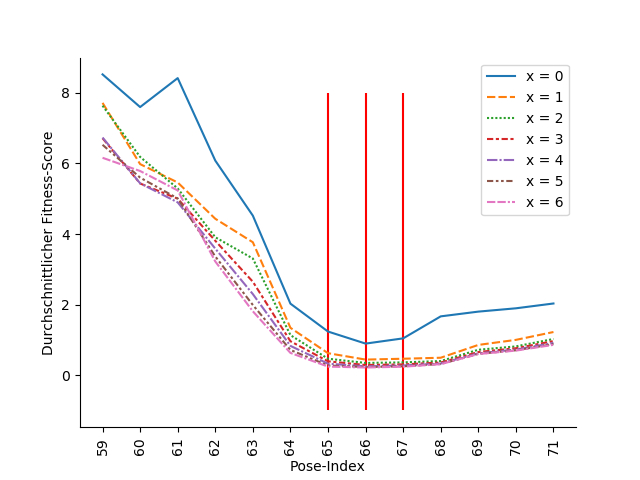
\includegraphics[width=.95\linewidth]{Windows_small}
  		 \centering \caption{Durchschnittlicher Fitness-Score für gefundene Schleifenschluss-Kandidaten eines Datensatz von Pose $0$ bis Pose $80$, Posen ohne Kandidaten sind nicht dargestellt.}
  		 \label{fig:single_tsdf}
	\end{subfigure}%
	\begin{subfigure}{.5\textwidth}
    	\centering
  		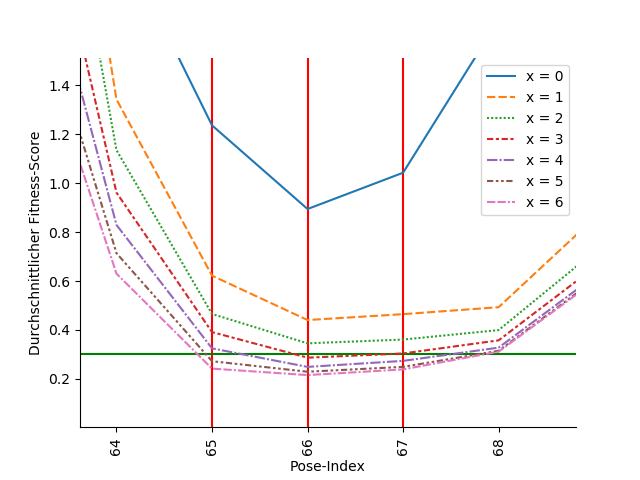
\includegraphics[width=.95\linewidth]{Windows_small_limit}
  		\centering \caption{Vergrößerung des Bereiches von links, in dem Schleifenschlüsse gefunden und validiert wurden. Dargestellt als grüne horizontale Linie ist die parametrisierte Schranke für Schleifenschlüsse.}
  		\label{fig:approx_cloud}
	\end{subfigure}
	\caption{Diese Grafik zeigt den Einfluss des Fensters für die Anreicherung der Model-Punktwolke bei der Validierung gefundener Schleifenschluss-Kandidaten, gegeben die Größe des Fensters $x$. Rote vertikale Linien markieren Posen, an den Schleifenschlüsse detektiert und aufgrund des geringen Fitness-Scores validiert wurden. Die Gesamtmenge der Posen, deren Punktwolken zu einer dichteren Model-Punktwolke zusammengeführt werden, beträgt $2 \cdot x + 1$. Es ist zu erkennen, dass der durchschnittlich berechnete Fitness-Score mit steigendem $x$ im Schnitt niedriger ist. Allerdings wird die Verringerung ab einem gewissen Punkt unwesentlich. Hier sind zwischen einer Wahl von $x = 2$ bis $x = 6$ nur geringe Unterschiede zu erkennen. Die Größten Veränderungen sind zwischen $x = 0$ und $x = 2$ zu erkennen. Hier sinkt der durchschnittliche Fitness-Score merklich. Dies trifft auch auf die Ergebnisse im Scan-Matching zu. Diese verbessern sich bei zunehmendem $x$, hier sind ebenfalls die größten Veränderungen zwischen $x=0$ und $x=2$ zu sehen. Die Wahl des Fenster korreliert zusätzlich mit dem durchschnittlichen absoluten Fehler zwischen der durch die Schleifenschlüsse optimierten Trajektorie eines Datensatz und der zugehörigen \emph{Ground-Truth}.}
	\label{fig:Windows}
\end{figure}

Ein weiteres bereits angeschnittenes Problem sind Schleifenschlüsse, die zwar die vorgegebenen Rahmenbedingungen erfüllen, allerdings grundsätzlich fehlerhaft sind. Hier ist zum Beispiel in einem Flur das Scan-Matching aufgrund einer sehr Feature armen Umgebung konvergiert und die Validierung auf Basis des Fitness-Scores konnte zusätzlich keinen Fehler bei der Registrierung identifizieren. Dann werden häufig Posen, die in einer initialen Schätzung weit auseinander liegen aufeinander gezogen. Zusätzlich kann es vorkommen, dass das Scan-Matching mit einem guten Fitness-Score konvergiert, obwohl die Umgebungen nicht zueinander passen. Die berechnete finale Transformation ist in diesem Fall so fehlerhaft, dass sie nicht mit der initialen Schätzung vereinbar ist. Aus diesem Grund wurden zwei Validatoren beziehungsweise \emph{Rejector} entwickelt, die neben dem Fitness-Score zusätzliche Validations-Stufen einführen. Dies ist zum einen der \emph{Linien-Rejector} und auf  der anderen Seite der \emph{Reichweiten-Rejector}. Diese nutzen die Unsicherheiten der einzelnen Posen aus. Vor Beginn das Algorithmus erfolgt eine Einschätzung über die Sicherheit der initial bestimmten Posen. Diese kann beliebig schlecht gewählt werden um sicherzustellen, dass bei der Optimierung gewünschte Änderungen vorgenommen werden. Dies erhöht allerdings die Wahrscheinlichkeit für fehlerhafte Schleifenschlüsse, die durch die beiden im Folgenden beschriebenen Validatoren nicht erfasst werden können. Kann für eine Initial-Schätzung zum Beispiel aufgrund voriger Erfahrungen ein gewisser Fehler für die Translation und Rotation zwischen aufeinander folgenden Posen abgeschätzt werden, sollte dieser im Folgenden verwendet werden. Die Notwendigkeit einer solchen Evaluationsstufe wird unter anderem in \cite{tsintotas2022revisiting} und \cite{xie2017graphtinker} herausgestellt. Beide Papiere beschreiben, dass die Nutzung einer fehlerhaften Schleifenschlusses verhängnisvolle Auswirkungen auf das Ergebnis der Optimierung des Pose-Graphs hat. Diese Einschätzungen decken sich mit den hier festgestellten Bobachtungen.

\textbf{\textsl{Linien-Rejector}}

Je nach Parametrisierung ist es möglich, dass Schleifenschlüsse zwischen Posen $P_{cur}$ und $P_{prev}$ identifiziert werden, deren Zwischen-Posen näherungsweise auf einer Linie liegen. Der maximale Abstand einer Zwischen-Pose zur durch $P_{cur}$ und $P_{prev}$ definierten Linie ist mit $d_{line}$ definiert und parametrisierbar. Standardmäßig ist $d_{line} = 0.5m$. Eine beschriebene Identifikation ist im Regelfall möglich, wenn, wenn $d_{max} > d_{trav}$. In Ausnahmefällen kann dies bei bestimmten Trajektorien schon für geringere $d_{trav}$ der Fall sein. Diese Art von Schleifenschlüssen stellt im Grundsatz kein Problem dar, allerdings ist es durch die Bewertung des Ergebnisses des Scan-Matching anhand des Fitness-Scores besonders in Fluren oder ähnlichen Regionen, die unvorteilhaft für ein Scan-Matching sind, möglich, dass am Schleifenschluss beteiligte Posen ohne Rücksicht auf die initialen Schätzungen und Zwischen-Posen aufeinander gezogen werden. Abbildung \ref{fig:Line-Rejector} zeigt dieses dies schematisch und nimmt zusätzlich Bezug auf die Identifikation von diesen besonderen Fällen.

\begin{figure}
		\centering
		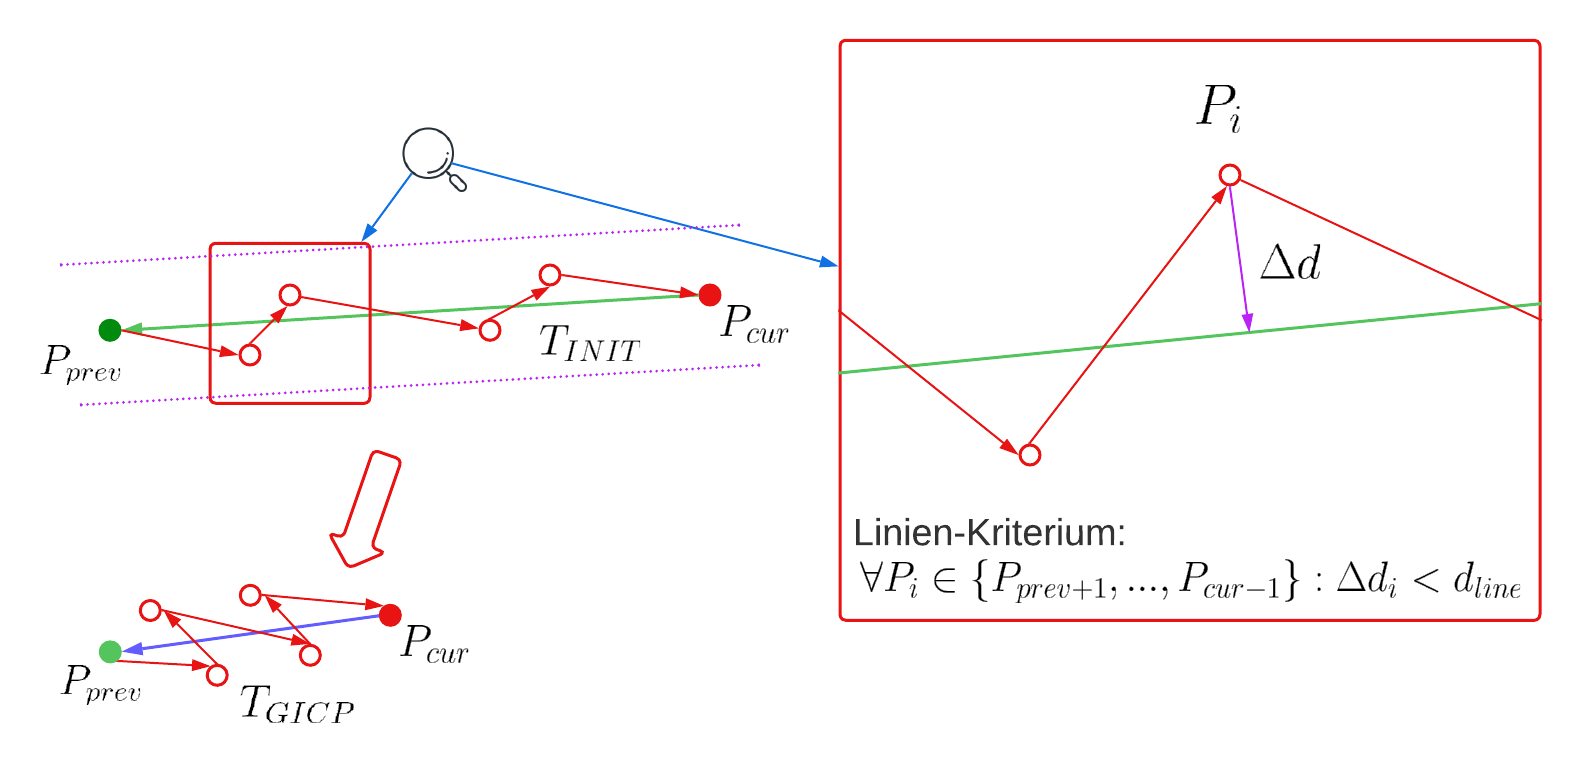
\includegraphics
			[scale=0.27]
			{Line-Rejector}
		\caption
			[Caption for LOF]{Diese Grafik beschreibt die Funktionsweise des Linien-Rejectors. Zusätzlich definiert sie das mathematische Kriterium für eine approximative Linie, gegeben $d_{line}$: $\forall P_i \in \left\lbrace P_{prev + 1}, ..., P_{cur - 1} \right\rbrace : \Delta d_i < d_{line}$. Die Abbildung ist zweigeteilt. In der rechten Vergrößerung eines Teilbereichs der oben links dargestellten Trajektorie ist das Linien-Kriterium dargestellt. Die Linie zwischen den beiden Posen $P_{cur}$ und $P_{prev}$ ist oben links und in der Vergrößerung in grün dargestellt. Sie wird durch den Translationsanteil von $T_{init}$, der initial gegebenen Transformation zwischen $P_{cur}$ und $P_{prev}$, sowie den Translationsanteil von $P_{cur}$ als Stützvektor gegeben. Durch lila gestrichelte Linien ist die Umgebung dargestellt, in der sich das Sensorsystem befindet. In diesem Fall handelt es sich um einen besonders Feature-armen Flur. Bei der Validierung mittels Scan-Matching (in diesem Fall per GICP) wurde die durch $T_{GICP}$ beschriebene Transformation ermittelt. In diesem Fall ist das Scan-Matching mit einem sehr guten Fitness-Score konvergiert, obwohl die Transformation Augenscheinlich fehlerhaft ist. Dies liegt an der beschriebenen Umgebung, die aus Sicht des Laserscanners für verschiedene Posen sehr ähnlich, wenn nicht nahezu identisch aussieht. Dies sind sehr schlechte Voraussetzungen für ein Scan-Matching. Unten links ist die zu erwartende Optimierung der Trajektorie auf Basis der fehlerhaften Transformation $T_{GICP}$. Bei den Zwischen-Posen tritt durch die Stauchung der Geraden ein Ziehharmonika-Effekt auf. Dies hat fatale Auswirkungen auf die generierte Karte und den weiteren Verlauf der Trajektorie.}                                                                                                                                     
		\label{fig:Line-Rejector}
\end{figure}

Wie zuvor beschrieben ist eine mögliche Lösung dieses Problems die Ausnutzung von relativen, lokalen Unsicherheiten zwischen aufeinanderfolgenden Posen. Der Linien-Rejector nutzt dabei die definierten Unsicherheiten für die Translation als Vektor aus den gegebenen Standardabweichungen: $\vec{\sigma_t} = \left(\sigma_x, \sigma_y, \sigma_z \right)$. Diese können entweder konstant gegeben oder für jede Pose-Differenz aufeinander folgender Posen einzeln, zum Beispiel anhand von Berechnungen im SLAM Ansatz, gegeben sein. Im Folgenden werden die Standardabweichungen als konstant angenommen. Gegeben $P_{cur}$ und $P_{prev}$, die Anzahl an Zwischen-Posen $N_{between}$, sowie die konstante Standardabweichung der Translation $\vec{\sigma_t}$ lässt sich nun Konfidenzintervall berechnen, in dem basierend auf der gegebenen Standardabweichung ein gewisser Prozentsatz der für $P_{cur}$ möglichen liegt. Dies ist in 3D ein räumlicher Bereich. Als Erwartungswert wird die initiale Schätzung für $P_{cur}$, genauer gesagt dessen Translationsanteil $\vec{t_{cur}}$ verwendet. Damit ergibt sich für die untere Grenze $\vec{t_u}$ und obere Grenze $\vec{t_o}$ des Konfidenzintervalls unter Ausnutzung der akkumulierten Standardabweichungen zwischen $P_{prev}$ und $P_{cur}$:

\begin{myequation}
\vec{t_u} = \vec{t_{cur}} - \left( N_{between} + 1 \right) \cdot k \cdot \vec{\sigma_t}
\end{myequation}

\begin{myequation}
\vec{t_o} = \vec{t_{cur}} + \left( N_{between} + 1 \right) \cdot k \cdot \vec{\sigma_t}
\end{myequation}

Dabei bezeichnet $k$ die verwendete standardisierte Intervallgrenze. Im Folgenden wird hierfür $1$ verwendet, eine beliebige Anpassung dieses Wertes ist möglich. Für $k=1$ werden für eine gegebene Standardabweichung im Konfidenzintervall etwa $80\%$ bis $85\%$ der möglichen relativen Pose-Änderungen zwischen aufeinander folgenden Posen abgedeckt. Der Prozentsatz des durch $\vec{t_u}$ und $\vec{t_o}$ abgedeckten Volumens berechnet sich aus folgender Potenz:

\begin{myequation}
\prod_{i=0}^{N_{between}} 0.8
\end{myequation}

Zugrunde liegt die Schätzung des Prozentsatzes, der durch die Intervallgrenzen, gegeben $k$ abgedeckt wird (hier etwa $80\%$). Für $4$ Zwischen-Posen beträgt die Abdeckung in diesem Fall in etwa $33\%$. Für eine größere Abdeckung ist ein größeres $k$ zu wählen. Mit zunehmender Anzahl an Zwischen-Posen wird der durch den Rejector abgedeckte Bereich verhältnismäßig immer kleiner, obwohl er linear vergrößert wird. Dies hat eine sehr strenge Behandlung von Schleifenschlüssen auf Linien zur Folge. Mit einem größeren $k$ kann dies entschärft werden. Liegt $P_{cur}$ nach Bestimmung der neuen Transformation $T_{GICP}$ außerhalb des durch $\vec{t_u}$ und $\vec{t_o}$ beschriebenen Volumens, der gefundene Schleifenschluss als ungültig angesehen. Liegt die neue Pose innerhalb des Volumens, ist sie validiert. Auf diese Weise konnten in einem Beispieldurchlauf für eine Fenster-Größe von $x = 0$ und $\Delta d = 2.0m$ bei einem Datensatz mit $200$ Posen $8$ fehlerhafte Schleifenschlüsse identifiziert und verworfen werden. Mit größerer Fenstergröße reduziert sich die Anzahl dieser fehlerhaften Schleifenschlüsse. So konnten bereits bei einer Größe von $x = 2$ in diesem Datensatz keine fehlerhaften Schleifenschlüsse identifiziert werden. Diese sind jedoch auch weiterhin nicht ausgeschlossen, weshalb der Rejector als weitere Sicherheitsschranke hinter das Scan-Matching geschaltet wird.

\textbf{\textsl{Reichweiten-Rejector}}

Der \emph{Reichweiten-Rejector} basiert auf dem identischen Prinzip wie der zuvor erläuterte Linien-Rejector. Hier wird zusätzlich zur Standardabweichung in der Translation auch die Standardabweichung in der Rotation berücksichtigt. Zusätzlich ist das Vorhandensein einer Linie keine Voraussetzung für diesen Rejector. Alle anderen mathematischen Verhältnisse aus dem oben vorgestellten Rejector treffen so auch hier zu und werden analog sowohl für die Translation, als auch für die Rotation angewandt.  Dieser Rejector ist dem Linien-Rejector nachgeschaltet. Der nachfolgende Abschnitt beschäftigt sich mit der Optimierung des Pose-Graphen auf Basis identifizierter Schleifenschlüsse unter zusätzlicher Validierung durch die soeben vorgestellten Validatoren.

\section{Optimierung des Pose-Graphen}

Für die Optimierung des Pose-Graphen wird in diesem Fall die C++ Bibliothek GTSAM \cite{dellaert2012factor} verwendet. GTSAM implementiert die Fusion von Sensor Daten für Anwendungen im Bereich von Robotik und Computergrafik und kommt insbesondere in SLAM-Ansätzen zum Einsatz \cite{dellaert2012factor}. Als unterliegende Datenstruktur für den hier verwendeten Anwendungsfall dient ein Faktorgraph. Faktorgraphen sind grafische Modelle, die sich gut für komplexe Schätzungsprobleme wie SLAM und deren Modellieren eignen. Ein Faktorgraph ist ein bipartiter beziehungsweise paarer Graph, der Beziehungen zwischen zwei Mengen darstellt. Der Graph besteht das Faktoren beziehungsweise \emph{Graph-Constraints}, die mit der Menge der \emph{Variablen} verbunden sind. Dabei stellen die Variablen die unbekannten Zufallsvariablen des Schätzproblems dar, während die Faktoren probabilistische Beschränkungen oder Voraussetzungen für diese Variablen darstellen, die aus Messungen wie Odometrie, \emph{IMU (Intertial Measurement Unit)}-Schätzungen, gesichteten Landmarken oder SLAM-Schätzungen abgeleitet werden \cite{dellaert2012factor}. Im Folgenden sind die Zufallsvariablen des Schätzproblems die gesuchten optimierten Posen des Pose-Graphs. Die mit GICP optimierten initialen Pose-Schätzungen, sowie die identifizierten Schleifenschlüsse werden als Faktoren verwendet. GTSAM stellt für diese Faktoren vordefinierte Klassen, die in Tabelle \ref{table:gtsam_faktoren} vorgestellt werden.

	\begin{table}
		\centering
		\caption{Verwendete GTSAM-Faktoren und deren Funktionsweise.}
		\begin{tabular}{| p{1.7cm} | p{8cm} | p{4cm} |}
			\hline
			\thead{Faktor}   & \thead{Beschreibung}  & \thead{Nutzung}\\
			\hline
			\textbf{Prior-Faktor}   & Definiert ein initiales Rauschen für die erste Pose des Pose-Graphen. Dieser Faktor ist der einzige verwendete Faktor, der einen absoluten Pose-Constraint beziehungsweise Faktor definiert. Alle anderen Faktoren sind relative Faktoren zwischen zwei Posen, gegeben durch ihre Indices. Aus diesem Grund wählt \cite{shan2020lio} an dieser Stelle ein großes initiales Rauschen, um die Optimierung nicht durch eine zu statische erste Pose einzuschränken. \cite{shan2020lio} definiert einen 6D Varianz-Vektor, der die Varianzen der Rotations- und Translationskomponenten (in dieser Reihenfolge, in $rad^2$ und $m^2$) enthält. Dieser lautet wie folgt: $\left( 10^{-2}, 10^{-2}, \pi \cdot \pi, 10^8, 10^8, 10^8 \right)^T$. Dies wurde in dieser Arbeit zunächst übernommen und später parametrisierbar gemacht. Die in dieser Arbeit verwendeten Default-Werte lauten: $\left(10^{-2}, 10^{-2}, 10^{-2}, 0.064, 0.064, 0.064\right)^T$. Diese orientieren sich an dem Ansatz von \cite{HATSDF}. & Der Prior-Factor wird insgesamt einmal für das definierte initiale Rauschen der ersten Pose verwendet. \\
			\hline
			\textbf{Between-Faktor}    & Definiert einen relativen Pose-Constraint zwischen zwei Posen $P_i$ und $P_j$, gegeben durch deren Indices $i$ und $j$. Dieser Constraint ist gegeben als 3D Pose-Differenz, bestehend aus Rotation und Translation. Hierfür stellt GTSAM die Klasse $Pose3$ zur Verfügung. Auch für diesen Faktor kann neben dem relativen Constraint zwischen zwei Posen auch eine Unsicherheit definiert werden. Für aufeinanderfolgende Posen ist diese parametrisch gegeben (Default: $\left(10^{-2}, 10^{-2}, 10^{-2}, 0.064, 0.064, 0.064\right)^T$), für identifizierte Schleifenschlüsse wird der beim Scan-Matching resultierende Fitness-Score $\Gamma$ verwendet: $\left(\Gamma, \Gamma, \Gamma, \Gamma, \Gamma, \Gamma\right)^T$. Bei dieser Entscheidung wurde sich an \cite{shan2020lio} orientiert. & Dieser Faktor findet sowohl zur Beschreibung der Pose-Differenzen aufeinanderfolgender Posen (gegeben durch die gegebenenfalls mit GICP optimierte, initiale Schätzung), als auch für die Beschreibung der im Scan-Matching ermittelten Pose-Differenz zwischen den an Schleifenschlüssen beteiligten Posen. \\
			\hline
		\end{tabular}
		\label{table:gtsam_faktoren}
	\end{table}	

In den Faktor-Graph selbst werden beim Durchlauf des Algorithmus lediglich die beschriebenen Faktoren eingefügt. Zu einem beliebigen Zeitpunkt besteht er aus dem initialen Prior-Faktor der ersten Pose, sowie mehren Between-Faktoren für aufeinander folgenden Posen und Schleifenschlüsse. Der Verbund mit der Menge der Variablen wird durch die Verwendung von Indices erreicht. Dabei erhält der Prior-Faktor den Index $0$, der er sich lediglich auf die erste Pose des Pose-Graphen bezieht, die mit $0$ indiziert ist. Between-Faktoren erhalten jeweils zwei Indices, die ebenfalls den entsprechenden Posen des Pose-Graphen zugeordnet werden können. Die beiden Indices legen fest, zwischen welchen Variablen der Faktor gilt und in welche Richtung er gilt. Der grundlegende Ablauf bei dem Einfügen neuer Faktoren in den Faktorgraphen und der anschließenden Optimierung der Variablenmenge, hier dem verwendeten Pose-Graphen, ist in Abbildung \ref{fig:Flussdiagramm-Optimization} dargestellt.

\begin{figure}
		\centering
		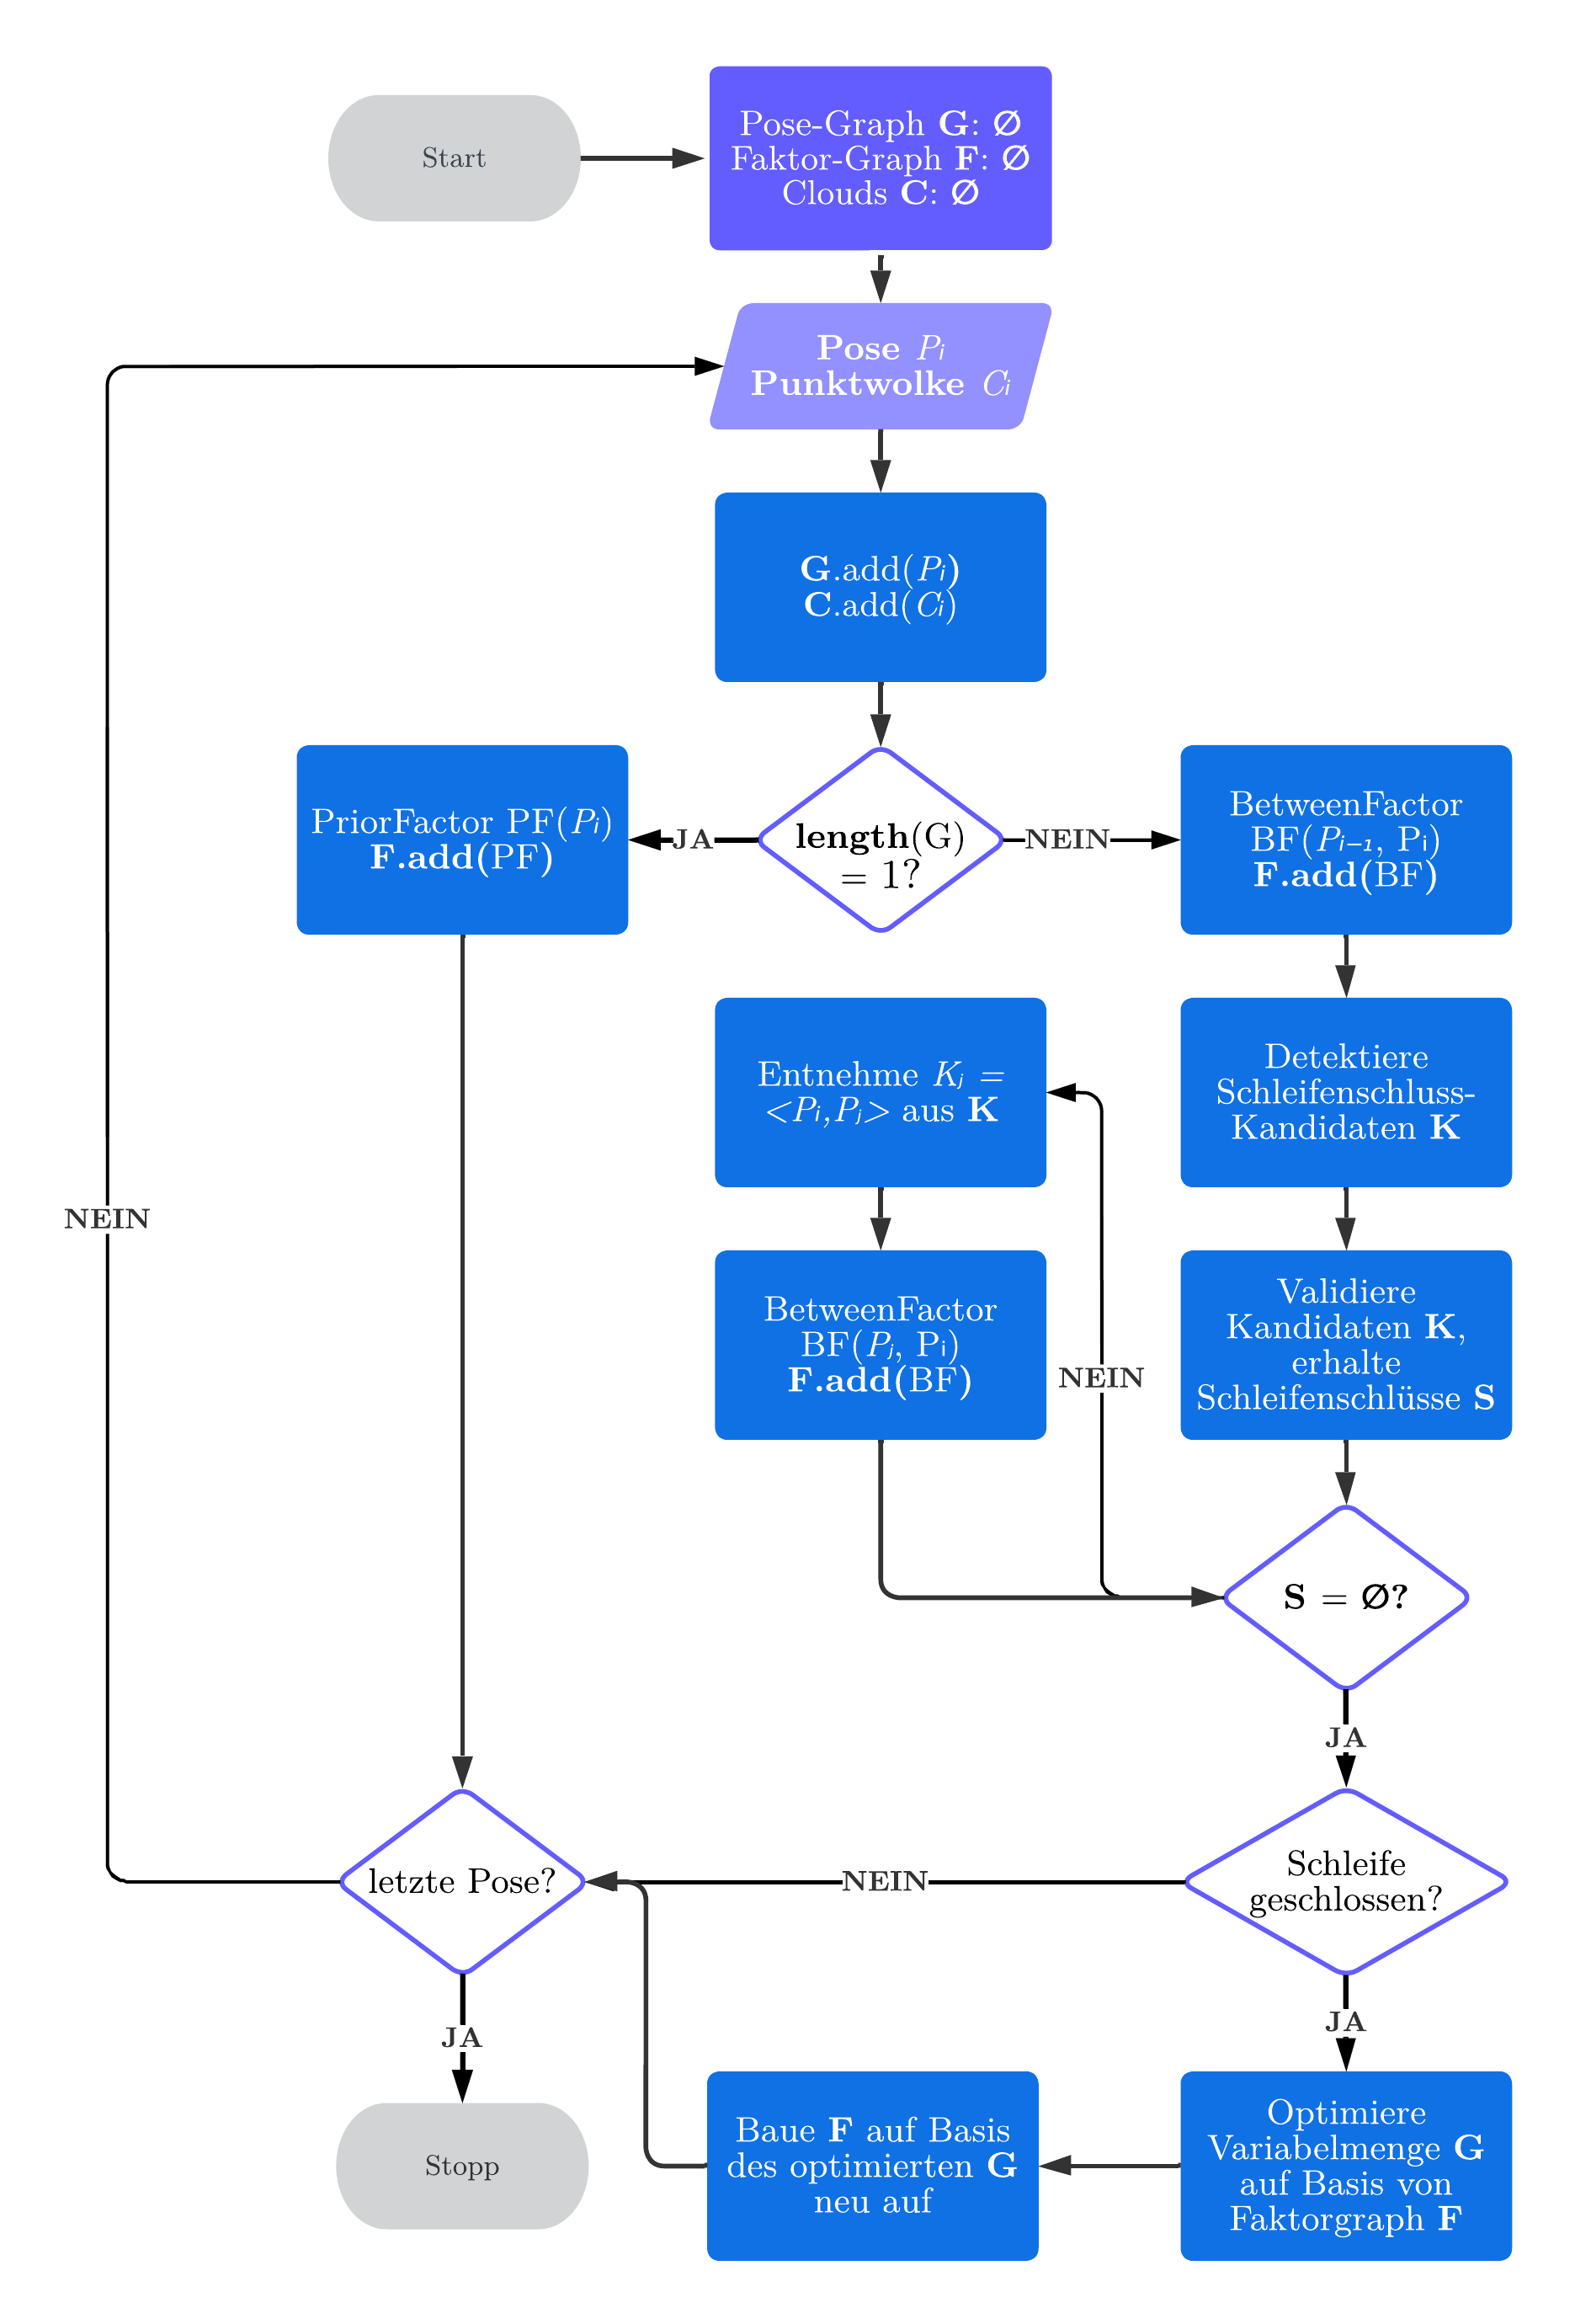
\includegraphics
			[scale=0.16]
			{Flussdiagramm-Optimization-colorized}
		\caption
			[Caption for LOF]{Dieses Flussdiagramm beschreibt den algorithmischen Ablauf der Graph-Optimierung unter besonderer Betrachtung der in den Faktorgraphen einzufügenden Faktoren. Für den Fall, dass Schleifenschlüsse gefunden werden, wird die Menge der Variablen, hier der Pose-Graph auf Basis der in den Faktorgraphen eingefügten Faktoren optimiert. Als Optimierer wird hier der in GTSAM implementierte \emph{Levenberg-Marquardt-Optimizer} verwendet, der die von Levenberg \cite{levenberg1944method} und Marquard \cite{marquardt1963algorithm} vorgeschlagene Lösung von nicht-linearen \emph{Least-Squares} Problemen implementiert. Im Anschluss an die durchgeführte Optimierung, muss der Faktor-Graph $F$ auf Basis der neuen Pose-Differenzen in $G$ neu aufgebaut werden. Dies wird so lange durchgeführt, bis das letzte Pose-Punktwolke Paar der initialen Schätzung abgearbeitet ist. Um die Pose-Differenzen der initialen Schätzung auch nach der Optimierung des Teilgraphen beim Einfügen einer neuen Pose $P_i$ zu erhalten wird mit \emph{Pose-Deltas} gearbeitet. Dazu wird immer die zuletzt eingefügte Pose der initialen Schätzung gespeichert, bei einer neuen Pose das Pose-Delta beziehungsweise die Pose-Differenz zwischen der neuen und der gespeicherten Pose berechnet und auf die zuletzt eingefügte Pose in $G$ angewandt.}                                                                                                                                     
		\label{fig:Flussdiagramm-Optimization}
\end{figure}

Im Folgenden wird der hier vorgestellte Ansatz auf Basis mehrerer Datensätze evaluiert.

\section{Evaluation der Graph-Optimierung}

Dieser Absatz befasst sich mit der Evaluation des zuvor vorgestellten Ansatzes zur Optimierung des Pose-Graphen mittels identifizierter Schleifenschlüsse unter Verwendung der GTSAM Bibliothek \cite{dellaert2012factor}. Wie beschrieben werden zur Evaluation des Ansatzes mehrere Datensätze verwendet, die aus einer Initialschätzung des Pose-Graphen mit einer zu jeder Pose $P_i$ zugehörigen Punktwolke $C_i$, die relativ zum Koordinatensystem der zugehörigen Pose gesehen ist. Zu den verwendete Datensets gehört sowohl der \emph{Hannover-1} Datensatz der Universität Osnabrück mit zugehöriger Initialschätzung des Pose-Graphen durch Odometrie und einer \emph{Ground-Truth}, die in \cite{sprickerhof2011heuristic} vorgestellt wird. Die Ground-Truth bezeichnet eine Pose-Historie, die die (näherungsweise) realen Posen enthält, von denen die Daten aufgenommen wurden. Dies erlaubt einen direkten Vergleich der mit diesem Ansatz optimierten Trajektorie mit der Ground-Truth. Zusätzlich wurden im Laufe dieser Arbeit weitere Datensätze aufgenommen. Aus diesen Datensätzen erfolgte zunächst die Bestimmung einer Initialschätzung des Pose-Graphen mit einer überarbeiteten Variante des in \cite{zhang2014loam} vorgestellten SLAM-Ansatzes. Bei einer visuellen Überprüfung der so generierten Initialschätzungen fallen direkt mehrere Fehler wie doppelte Wände auf, die durch eine Fehlerfortpflanzung beim SLAM auftreten. Im Zuge dieser Evaluation soll überprüft werden ob diese Fehler durch diesen Ansatz kompensiert werden können.

\subsection{Datensatz: Hannover-1}

Zunächst erfolgt eine Evaluation des Hannover-1 Datensatzes, dessen Daten zunächst vom rechtshändischen ins linkshändische Koordinatensystem transformiert werden mussten. Abbildung \ref{GTvsInit} zeigt eine Gegenüberstellung der beschriebenen Ground-Truth des Datensatzes mit der durch Odometrie gegebenen Initialschätzung. Hier ist eine deutliche Differenz zwischen den beiden Pose-Graphen zu erkennen, die nicht ausschließlich durch die Integration von Schleifenschlüssen aufgelöst werden kann. Aus diesem Grund wird eine Vorregistrierung der aktuell betrachteten Initialschätzung der Pose $P_i$ mit den zuvor in den Pose-Graphen eingefügten Posen mittels GICP vorgenommen. Lediglich für die erste Pose wird die initiale Schätzung verwendet. Wie zuvor erläutert und in Abbildung \ref{fig:Windows} schematisch dargestellt ist , verbessert eine Anreicherung der Model-Punktwolke mit den Punktwolken der benachbarten Posen das Ergebnis der Registrierung maßgeblich. Diese Erkenntnis kommt auch bei der Vorregistrierung zum Einsatz. Der erörterte Vorregistrierungs-Schritt findet zusätzlich bei den anderen Datensätzen Verwendung, um eine lokale Konsistenz der Daten zu gewährleisten.


\begin{figure}
		\centering
		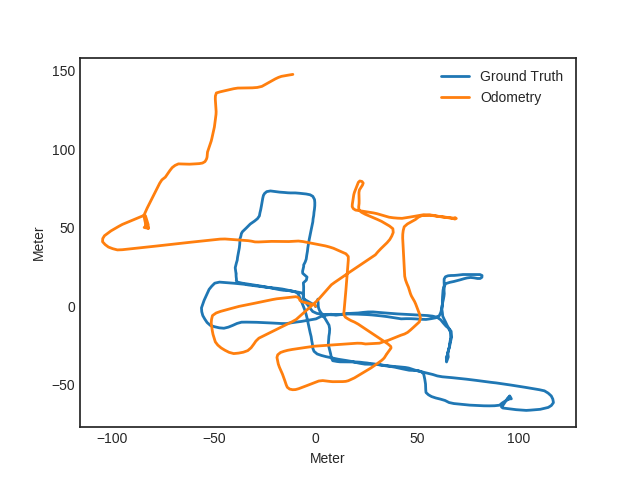
\includegraphics
			[scale=0.7]
			{GTvsInit}
		\caption
			[Caption for LOF]{Diese Grafik zeigt die Ground-Truth des Hannover-1 Datensatzes im Vergleich mit der initialen Odometrieschätzung. Es ist ersichtlich, dass die Odometrieschätzung signifikante Fehler aufweist, sodass die Trajektorien stark divergieren.}                                                                                                                                     
		\label{GTvsInit}
\end{figure}

\begin{figure}
		\centering
		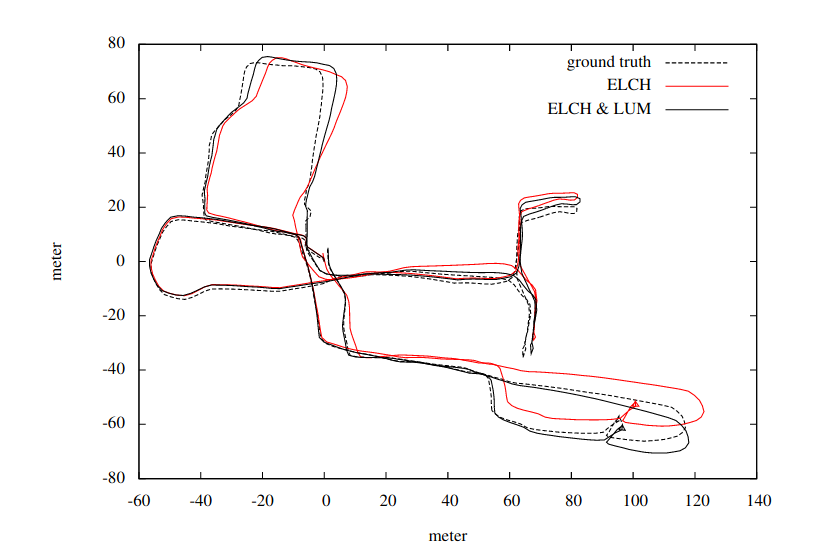
\includegraphics
			[scale=0.45]
			{elch}
		\caption
			[Caption for LOF]{Diese Grafik wurde aus \cite{sprickerhof2011heuristic} entnommen und dient als Vergleich zu den in Kapitel \ref{chapter:loop_closure} herausgearbeiteten Ergebnissen. Ein direkter, wertebasierter Vergleich mit den Ergebnissen aus \cite{sprickerhof2011heuristic} ist nicht möglich, da diese dort nur für einen anderen Datensatz angegeben sind. Ein visueller Vergleich der Ansätze zeigt aber eine deutliche Verbesserung des in dieser Arbeit vorgestellten Ansatzes im Gegensatz zum vorgeschlagenen Ansatz aus \cite{sprickerhof2011heuristic}. Nur an wenigen Stellen ist eine leicht größere Abweichung zur Ground-Truth zu erkennen. An allen anderen Stellen ist eine deutliche Verbesserung erkennbar.}                                                                                                                                     
		\label{fig:ELCH}
\end{figure}

Um die Effektivität der Schleifenschlüsse im hier vorgestellten Ansatz herauszustellen, erfolgt ein Vergleich mit einer Registrierung des Datensatzes durch GICP. Dies ist in Abbildung \ref{fig:Han1This} dargestellt. Zu erkennen ist eine deutliche Optimierung des Pose-Graphen durch die Einführung der Schleifenschlüsse. Lediglich eine Teilschleife des Graphen weicht im Vergleich stärker von der Ground-Truth ab. Hier lag zunächst ein großer Fehler in der Vorregistrierung vor, der von den identifizierten Schleifenschlüssen nur zum Teil korrigiert werden konnte. Dies wird hier zusätzlich anhand einer weiteren Grafik deutlich gemacht, die den absoluten Fehler in der Translation zwischen einer Pose $P_i$ des mit diesem Ansatz korrigierten Pose-Graphen mit der zugehörigen Pose $P_i^{GT}$ der Ground-Truth vergleicht. Siehe dazu Abbildung \ref{fig:Han1Error}. Dabei ist der absolute Fehler $\varepsilon_{abs}$ für die aktuelle Anzahl an Posen $n_{cur}$, sowie den Translationsanteilen der Posen des mit diesem Ansatzes korrigierten Pfades $\vec{t_i}$ und der Ground-Truth $\vec{t_i^{GT}}$  wie folgt definiert:

\begin{myequation}
\varepsilon_{abs} = \frac{\sum_{i=0}^{n_{cur}} \norm{\vec{t_i^{GT}} - \vec{t_i}}}{n_{cur}}
\end{myequation}

Die Abbildung \ref{fig:Han1Error} zeigt dabei die deutlichen Verbesserungen des absoluten Fehlers durch die Nutzung von GICP und die weitere Verbesserung durch die Nutzung von Schleifenschlüssen. Ein direkter Vergleich mit den Ergebnissen aus \cite{sprickerhof2011heuristic} ist an dieser Stelle nicht möglich, da diese nur für einen anderen Datensatz gegeben sind. Abbildung \ref{fig:ELCH} zeigt eine aus \cite{sprickerhof2011heuristic} entnommene Grafik, anhand derer ein visueller Vergleich mit den hier erzielten Ergebnissen ermöglicht wird. Es ist zu erkennen, dass der präsentierte Ansatz in diesem Datensatz an vielen Stellen genauer ist als der Ansatz aus \cite{sprickerhof2011heuristic}. Dies gilt auch für die Ergebnisse  basierend auf dem Nachbearbeitungsschritt, der die globale Optimierung des Pose-Graphen mit dem Ansatz von Lu \& Milios \cite{lu1997globally} realisiert.

\begin{figure}
	\centering
	\begin{subfigure}{.5\textwidth}
		 \centering
  		 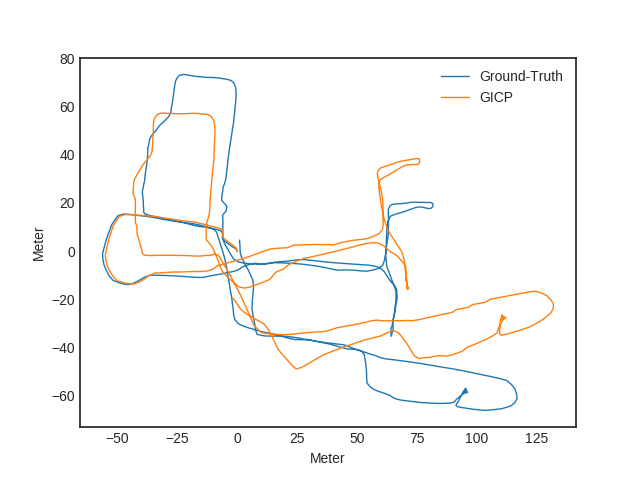
\includegraphics[width=1.0\linewidth]{GTvsGICP}
  		 \centering \caption{Vergleich einer Registrierung des Datensatzes mittels GICP, basierend auf den initial geschätzten Posen, mit der Ground-Truth.}
  		 \label{fig:Han1Initial}
	\end{subfigure}%
	\begin{subfigure}{.5\textwidth}
    	\centering
  		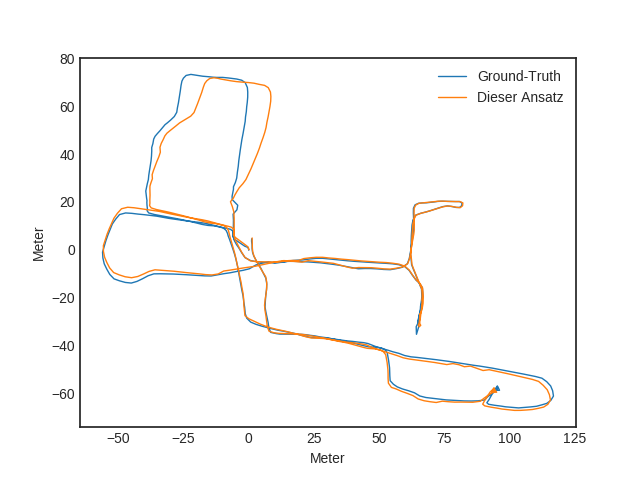
\includegraphics[width=1.0\linewidth]{GTvsThis}
  		\centering \caption{Vergleich des hier vorgestellten Ansatzes mit der Ground-Truth.}
  		\label{fig:Han1GT}
	\end{subfigure}
	\caption{Diese Grafik zeigt einen Vergleich des nur mit GICP registrierten Ergebnisses auf der linken Seite mit dem Ergebnis des hier vorgestellten Ansatzes, der neben einer Vorregistrierung mit GICP zusätzlich Schleifenschlüsse integriert, auf der rechten Seite. Beide Ergebnisse sind jeweils im Vergleich zur genannten Ground-Truth dargestellt. Es ist zu erkennen, dass die Registrierung des Datensatzes mittels GICP, basierend auf den initial geschätzten Posen eine deutliche Verbesserung erzielt, jedoch weiterhin große Abweichung zur Ground-Truth vorliegen. Der hier vorgestellte Ansatz nutzt die durch GICP vorregistrierten Daten und führt zusätzlich eine Optimierung des Graphen mittels Schleifenschlüssen ein. Dies verbessert das Ergebnis unter Betrachtung der Ground-Truth signifikant.}
	\label{fig:Han1This}
\end{figure}


\begin{figure}
	\centering
	\begin{subfigure}{.5\textwidth}
		 \centering
  		 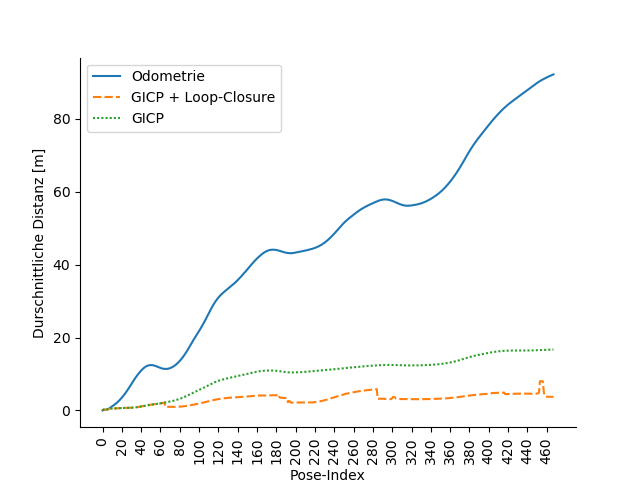
\includegraphics[width=1.0\linewidth]{initialVsGIPVsLC}
  		 \centering \caption{Vergleich des absoluten Fehlers $\varepsilon_{abs}$ zwischen der initialen Schätzung, des Pose-Graphen nach Registrierung mit GICP und dem Ergebnis des hier vorgestellten Ansatzes mit der Ground-Truth.}
  		 \label{fig:initialVsGIPVsLC}
	\end{subfigure}%
	\begin{subfigure}{.5\textwidth}
    	\centering
  		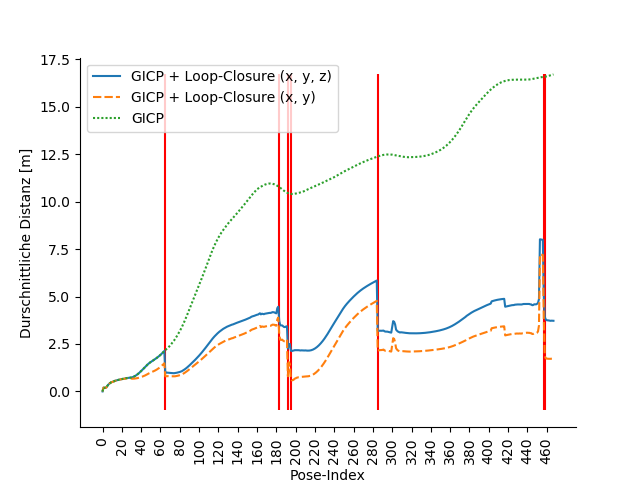
\includegraphics[width=1.0\linewidth]{GICPvsLC_error2}
  		\centering \caption{Vergleich des absoluten Fehlers $\varepsilon_{abs}$ zwischen ddem Pose-Graphen nach Registrierung mit GICP und dem Ergebnis des hier vorgestellten Ansatzes mit der Ground-Truth. Rote vertikale Linien zeigen dabei die Schleifenschlüsse durch die der absolute Fehler um mindestens $10\%$ reduziert wurde. Die absolute Anzahl an Schleifenschlüssen ist deutlich höher.}
  		\label{fig:GICPvsLC_error2}
	\end{subfigure}
	\caption{Diese Grafik vergleicht den absoluten Fehler $\varepsilon_{abs}$ in der Translation zwischen einer Pose $P_i$ mit der zugehörigen Pose $P_i^{GT}$ der Ground-Truth. Zusätzlich zum absoluten Fehler dieses Ansatzes wurde in der rechten Abbildung zusätzlich der absolute Fehler unter Vernachlässigung der z-Achse untersucht. Diese Untersuchung wurde so bereits in \cite{sprickerhof2011heuristic} durchgeführt, da der aufgenommene Datensatz aufgrund der Konfiguration des Sensorsystems bei der Registrierung aus unbekannten Gründen eine Kurvenform in der z-Achse annimmt. Aus diesen Grund wurde an dieser Stelle ebenfalls eine Projektion der Daten auf die $z=0$ Ebene vorgenommen und der entsprechende Fehler verglichen. Dieser ist mit einem durchschnittlichen absoluten Fehler von $1.7m$ deutlich geringer als der finale Fehler ohne die Projektion, der bei $3.7m$ liegt.}
	\label{fig:Han1Error}
\end{figure}

Im Folgenden wird der Ansatz auf Basis weiterer Datensätze der Universität Osnabrück validiert.

\subsection{Datensatz: Chemnitzer Opernhaus}

Ein weiterer Datensatz der Universität Osnabrück ist eine Aufnahme des Vorplatzes der Oper in Chemnitz. Grundlage für die Optimierung mit dem hier vorgestellten Ansatz ist eine Initialschätzung des Pose-Graphen mit einer abgewandelten Variante des in \cite{zhang2014loam} vorgestellten SLAM-Ansatzes. Ein Ausschnitt der zur Initialschätzung zugehörigen Punktwolke ist in Abbildung \ref{fig:chemnitz_double_walls} dargestellt. Hier wird aufgrund der gekennzeichneten doppelten Wände und Objekte deutlich, dass ein akkumulativer Fehler in der bestimmten Initialschätzung vorliegt. Dieser Fehler soll nun mit Hilfe des hier vorgestellten Ansatzes korrigiert werden. Dazu wird der Pose-Graph wie in Abbildung \ref{fig:Flussdiagramm-Optimization} vorgestellt optimiert. Das Ergebnis dieser Optimierung ist die in Abbildung \ref{fig:vorplatz_paths_3d} gekennzeichnete Anpassung des Pose-Verlaufs. Die Anpassung der Punktwolke auf Basis des korrigierten Pfades wird durch eine Transformation der zu $P_i$ zugehörigen Punktwolke $C_i$. Die dazu verwendete Transformation ist die Transformation von $P_i$ ins Koordinatensystem der Karte: $T_{P_i \rightarrow MAP}$. Das Ergebnis der Korrektur ist ebenfalls in Abbildung \ref{fig:chemnitz_double_walls} zu erkennen.

\begin{figure}
	\centering
	\begin{subfigure}{.5\textwidth}
		 \centering
  		 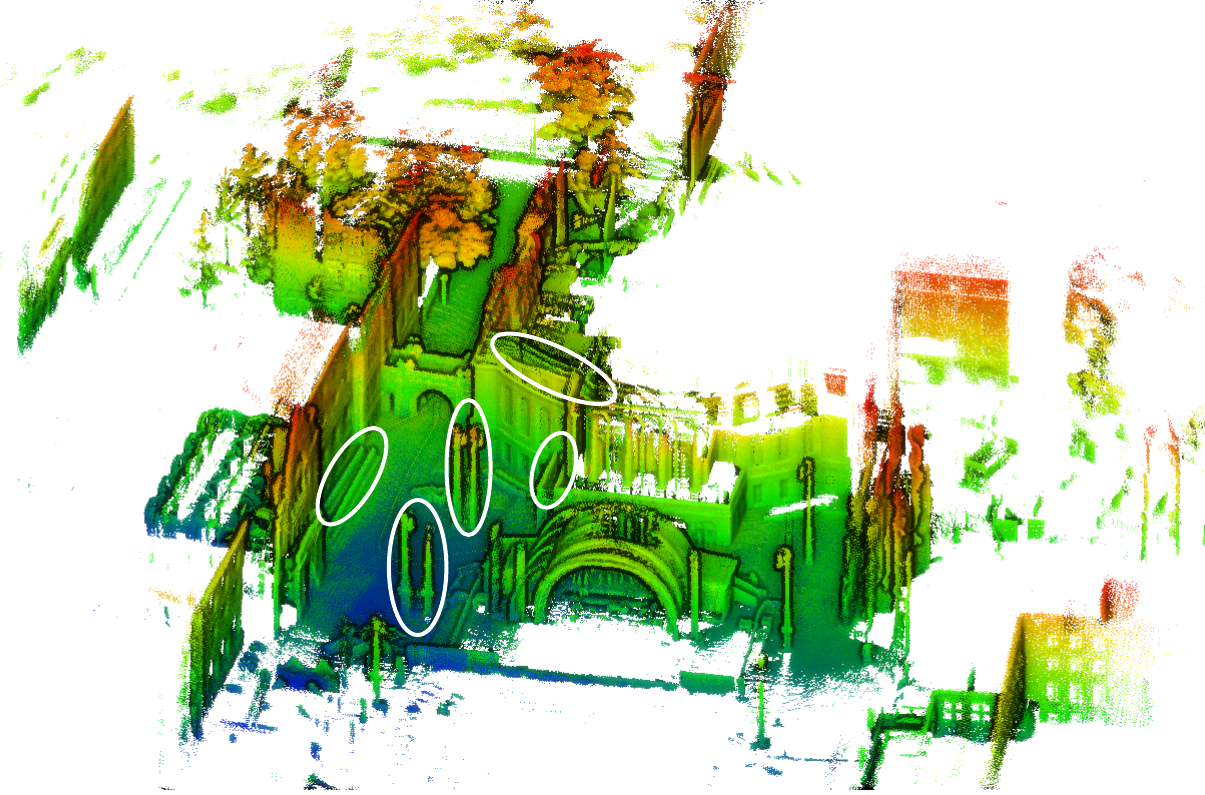
\includegraphics[width=1.0\linewidth]{double_walls_marked_white}
  		 \centering \caption{Punktwolke basierend auf der genannten Initialschätzung der Trajektorie.}
  		 \label{fig:double_walls_marked}
	\end{subfigure}%
	\begin{subfigure}{.5\textwidth}
    	\centering
  		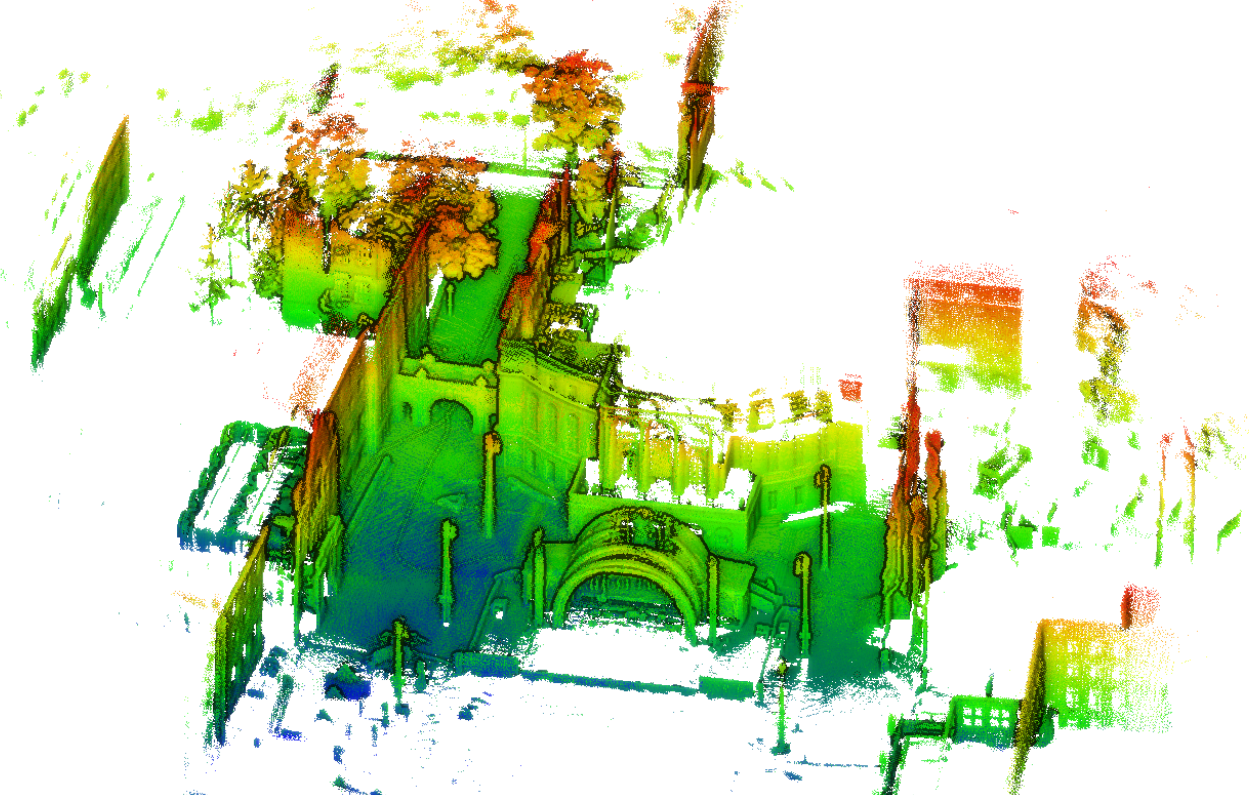
\includegraphics[width=1.0\linewidth]{no_double_walls_cut}
  		\centering \caption{Punktwolke basierend auf der mit dem hier vorgestellten Ansatz optimierten Trajektorie.}
  		\label{fig:no_double_walls_cut}
	\end{subfigure}
	\caption{Diese Grafik zeigt einen Vergleich der Punktwolken der Chemnitzer Oper vor und nach der in diesem Ansatz angewandten Korrektur. Zu erkennen ist eine deutliche Verbesserung des Gesamtbildes der Punktwolke durch die Nutzung der Schleifenschlüsse. Doppelte Wände durch akkumulative Fehler konnten nahezu vollständig kompensiert werden.}
	\label{fig:chemnitz_double_walls}
\end{figure}



\begin{figure}
	\centering
	\begin{subfigure}{.65\textwidth}
		 \centering
  		 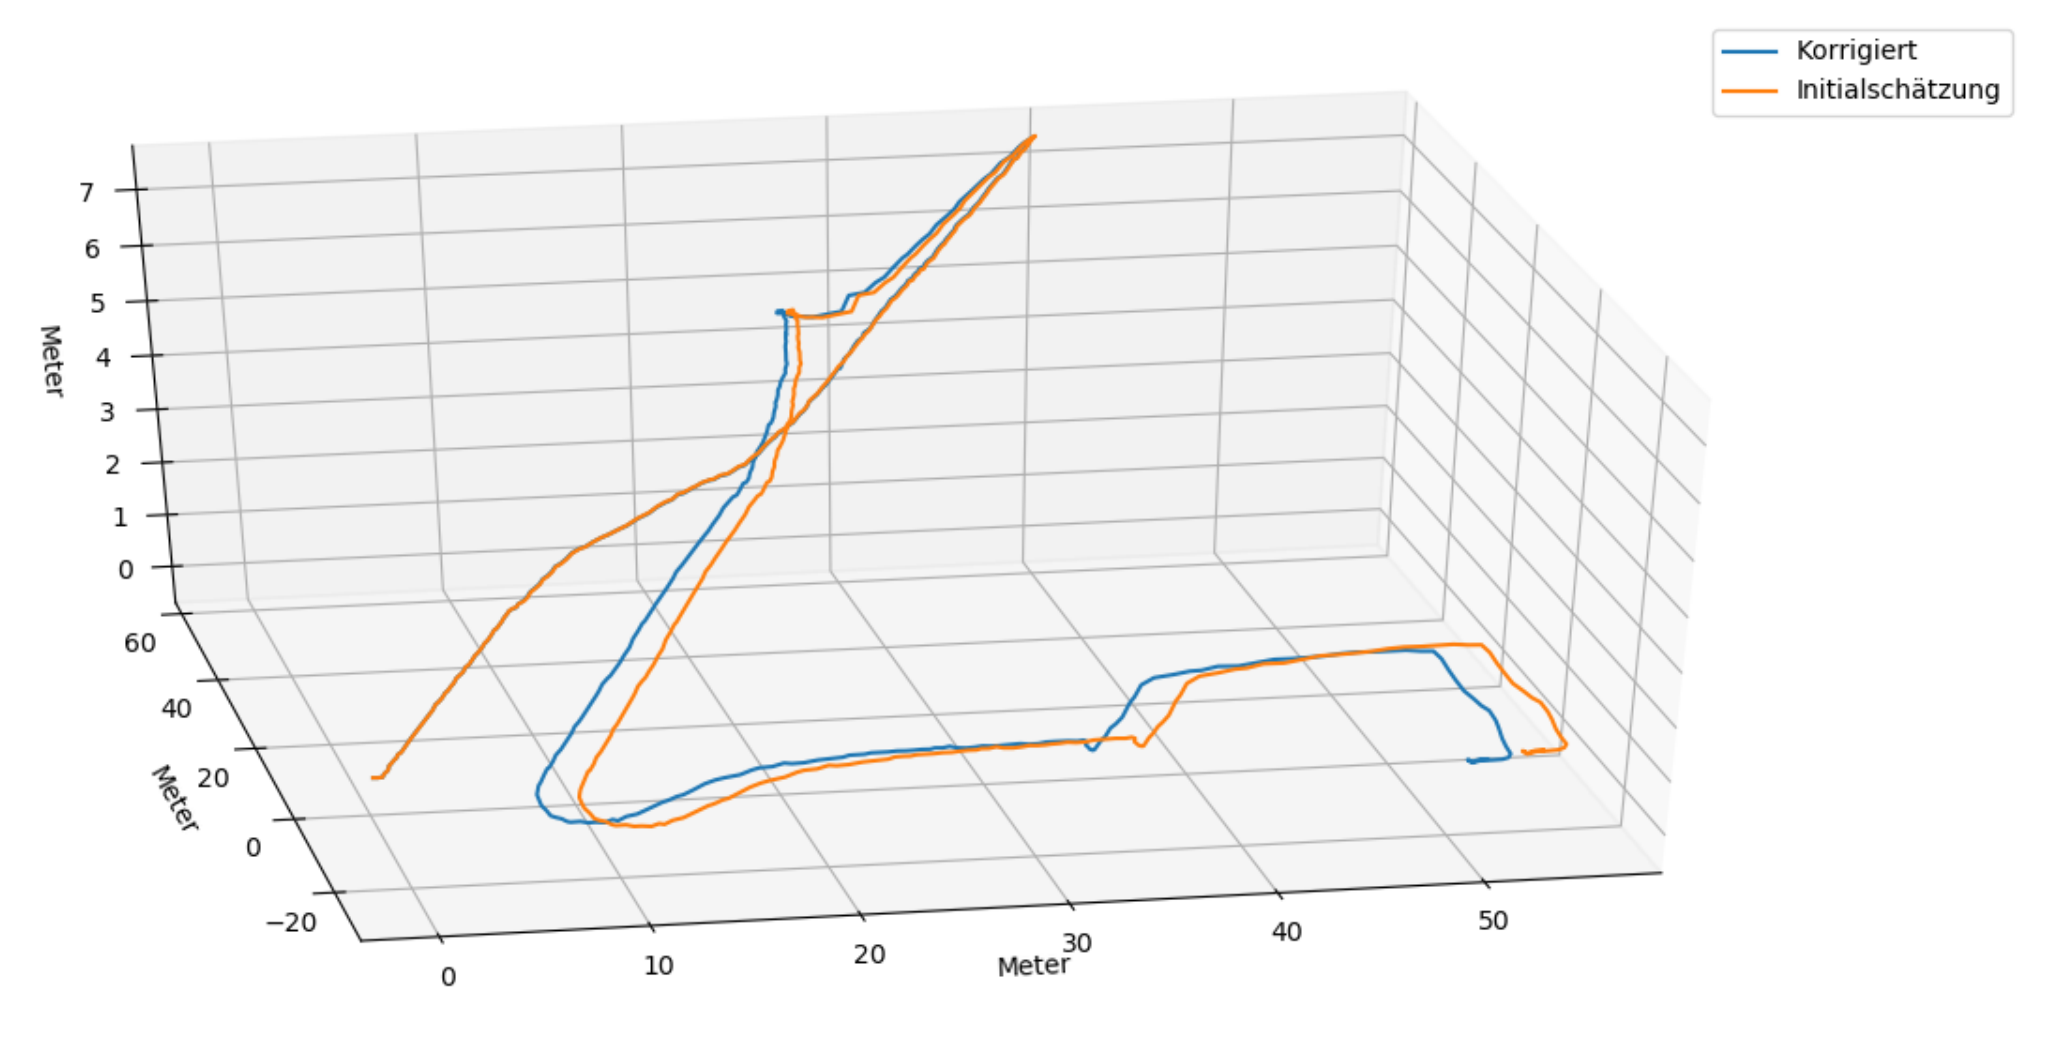
\includegraphics[width=1.0\linewidth]{vorplatz_paths_3d}
  		 \centering \caption{Vergleich zwischen Initialschätzung und Korrektur.}
  		 \label{fig:vorplatz_paths_3d1}
	\end{subfigure}%
	\begin{subfigure}{.35\textwidth}
    	\centering
  		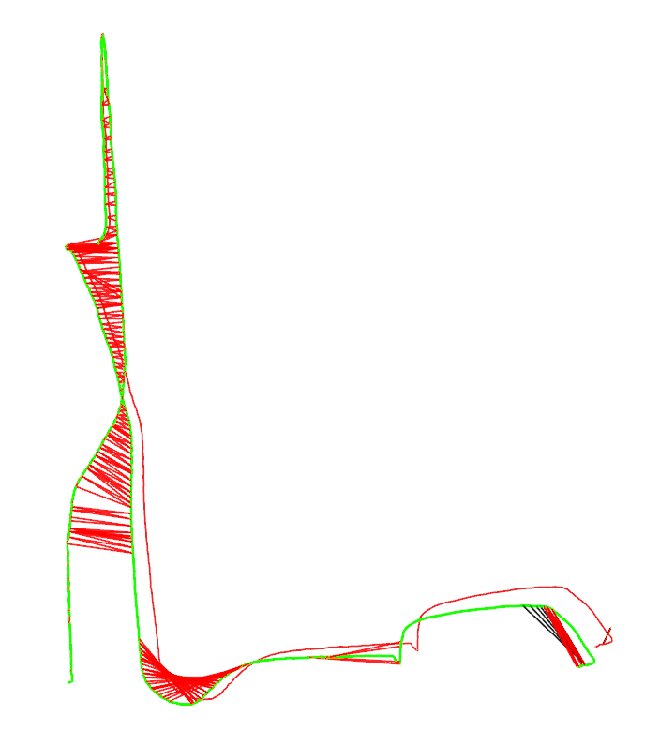
\includegraphics[width=1\linewidth]{chemnitz_no_lila_p}
  		\centering \caption{Vergleich zwischen Initialschätzung (rote Trajektorie) und Korrektur (grüne Trajektorie), inklusive der Darstellung von Schleifenschlüssen.}
  		\label{fig:chemnitz_no_lila}
	\end{subfigure}
	\caption{Im linken Teil der Abbildung ist die Initialschätzung der Trajektorie des Roboters im Vergleich mit dem korrigierten Pfad dargestellt. Es ist eine sichtbare Anpassung der Trajektorie zu beobachten. Diese Anpassung sorgt für die in Abbildung \ref{fig:chemnitz_double_walls} erkennbare Kompensation der Fehlerakkumulation und resultiert in einem signifikant besseren Ergebnis, welches keine erkennbaren doppelten Wände ausweist. Die schräge Ausrichtung des Pfades -- und damit zusammenhängend auch der Punktwolke -- im Raum beruht auf der schrägen Position des Laserscanners. Zum Zeitpunkt der Aufnahme der Daten wurde dieser leicht schräg auf dem Kopf der Person positioniert, die die Daten aufgenommen hat. Dies gilt ebenfalls für den in Abbildung \ref{fig:physik_paths_3d} dargestellten Verlauf des Pose-Graphen. Der rechte Teil der Abbildung zeigt ebenfalls den genannten Vergleich, zeigt aber zusätzlich die identifizierten und validierten Schleifenschlüsse, anhand derer die Graph-Optimierung durchgeführt wurde. Diese sind als rote Linien eingezeichnet.}
	\label{fig:vorplatz_paths_3d}
\end{figure}


\subsection{Datensatz: Campus Universität Osnabrück}

Bei diesem Datensatz handelt es sich um einen Teil des Physikgebäudes der Universität Osnabrück inklusive der Tiefgarage mit Durchgang. Die Evaluation dieses Datensatzes erfolgt entsprechend des vorigen Absatzes und ist in Abbildung \ref{fig:physik_double_walls} und \ref{fig:physik_paths_3d} dargestellt. Zu erkennen ist, dass auch hier eine Kompensation der Fehlerfortpflanzung durch den hier vorgestellten Ansatz erreicht werden konnte.

\begin{figure}
	\centering
	\begin{subfigure}{.5\textwidth}
		 \centering
  		 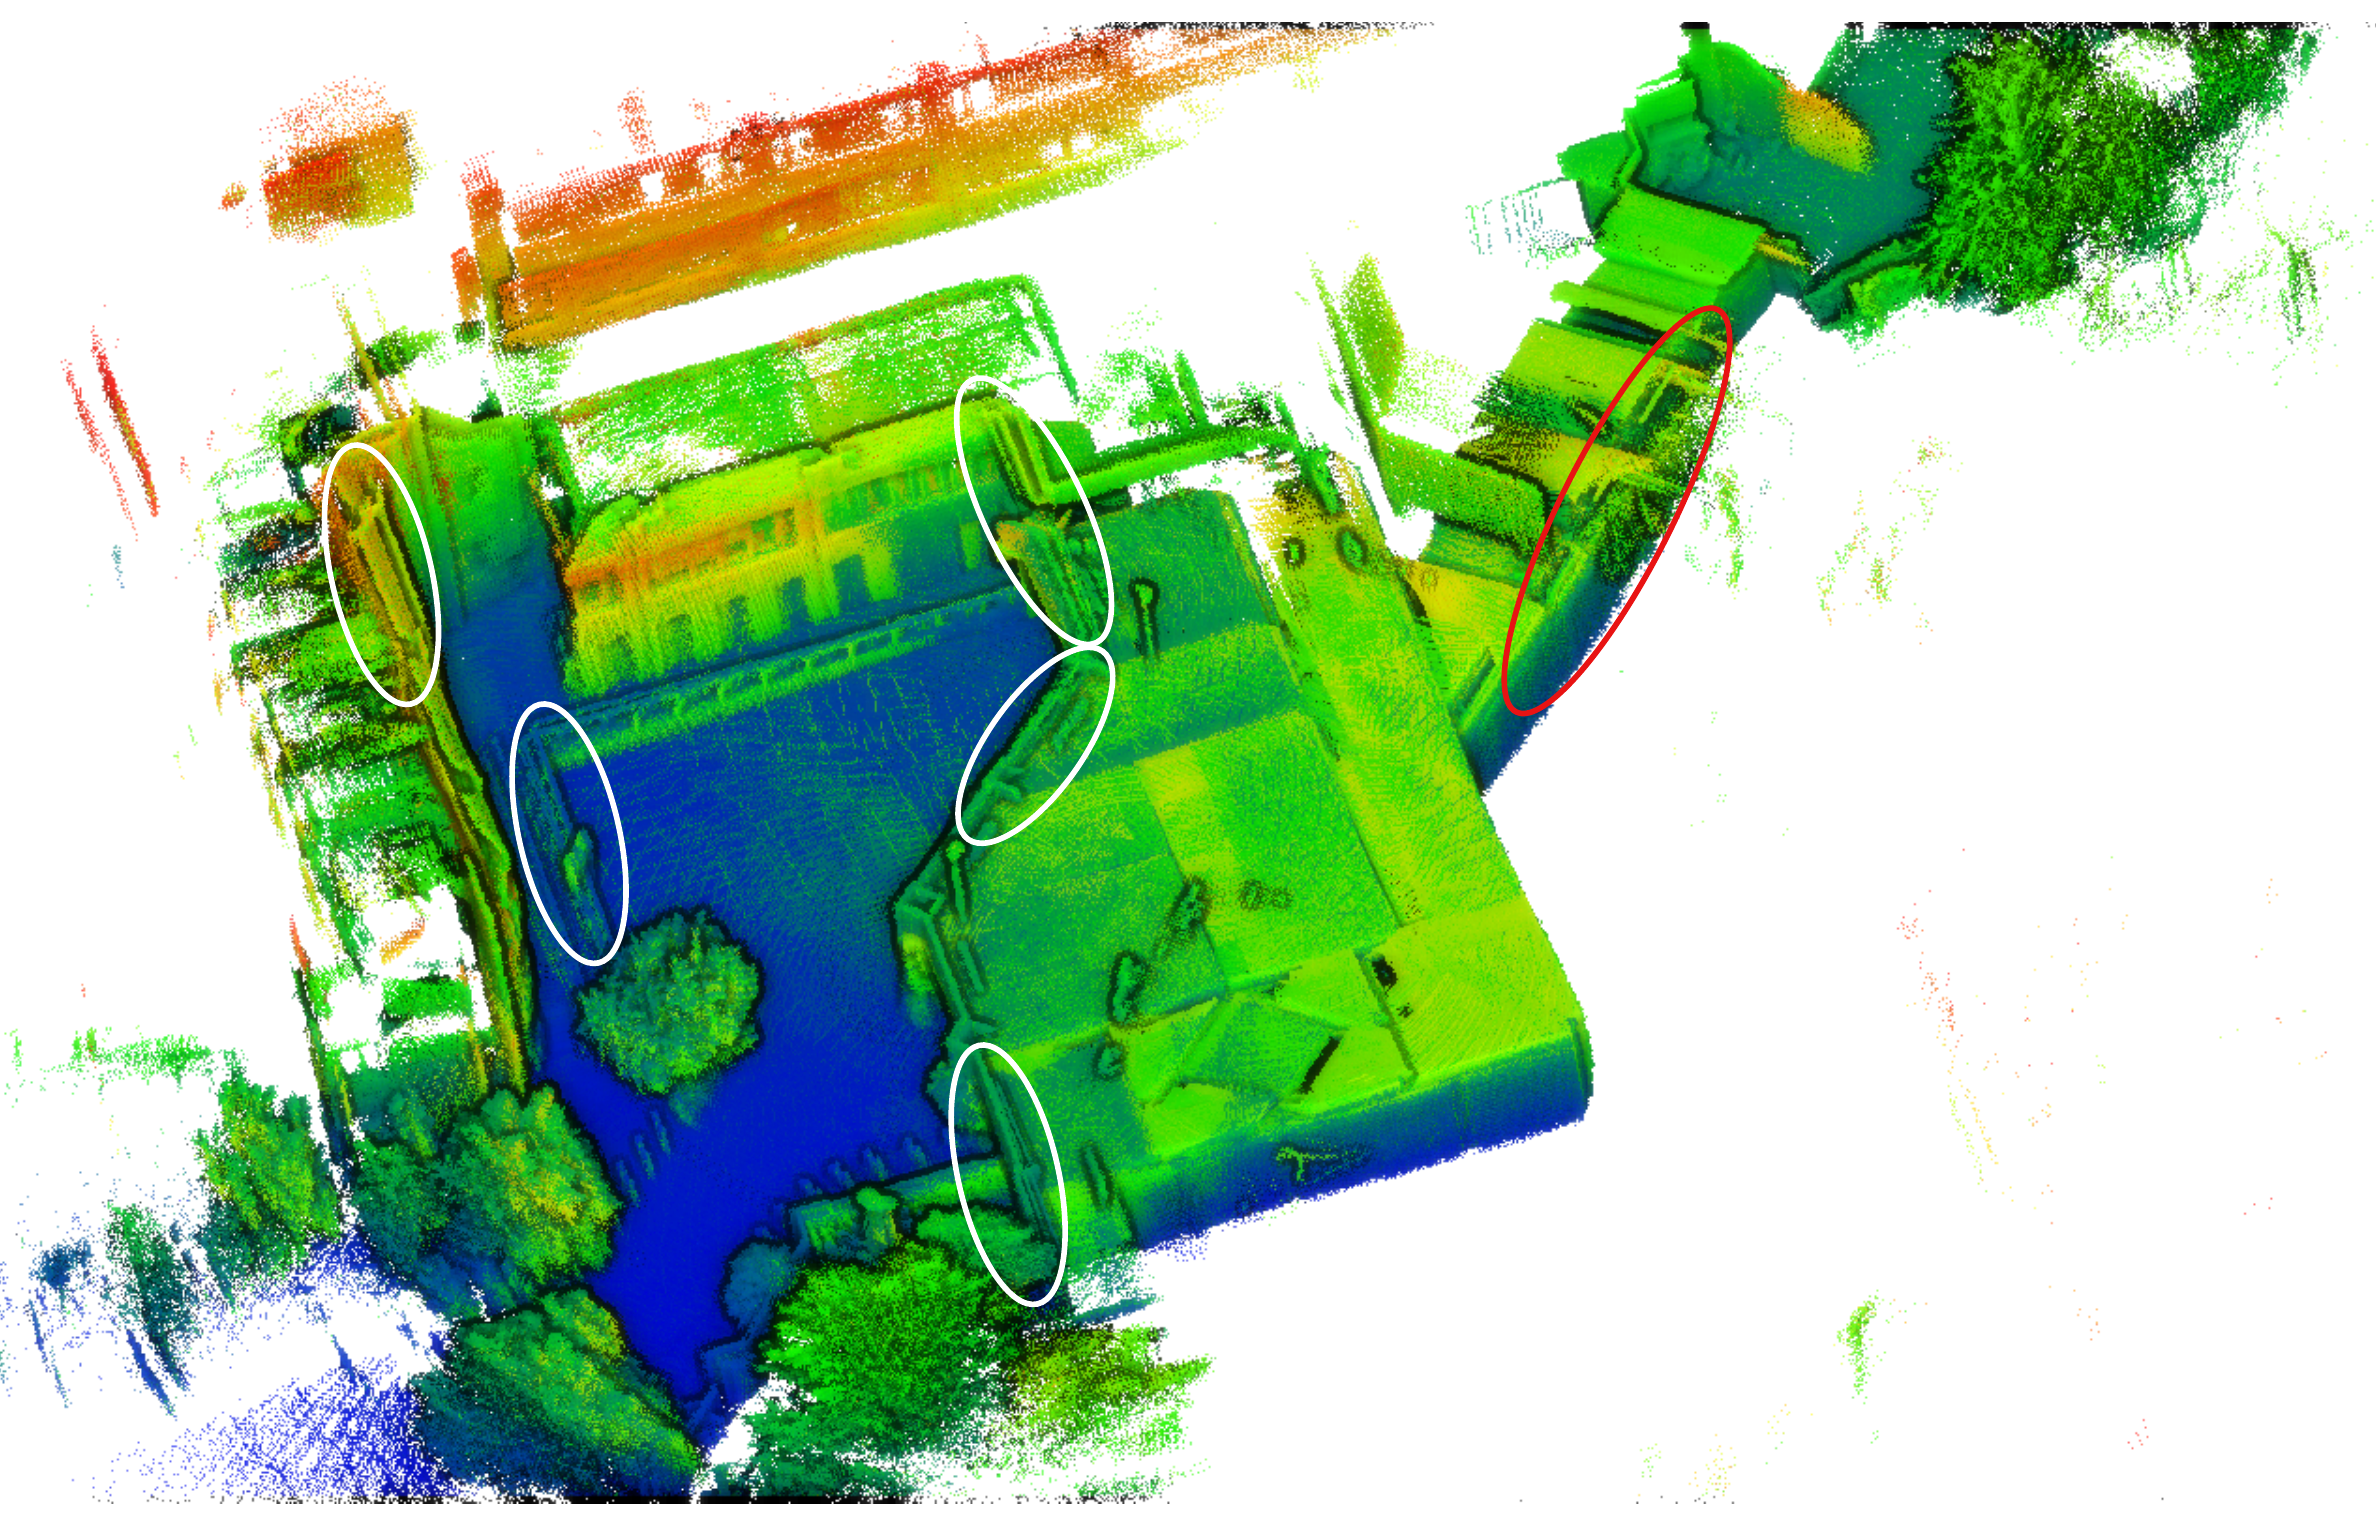
\includegraphics[width=1.0\linewidth]{physik_double_marked}
  		 \centering \caption{Punktwolke basierend auf der Initialschätzung der Trajektorie.}
  		 \label{fig:physik_double_walls}
	\end{subfigure}%
	\begin{subfigure}{.5\textwidth}
    	\centering
  		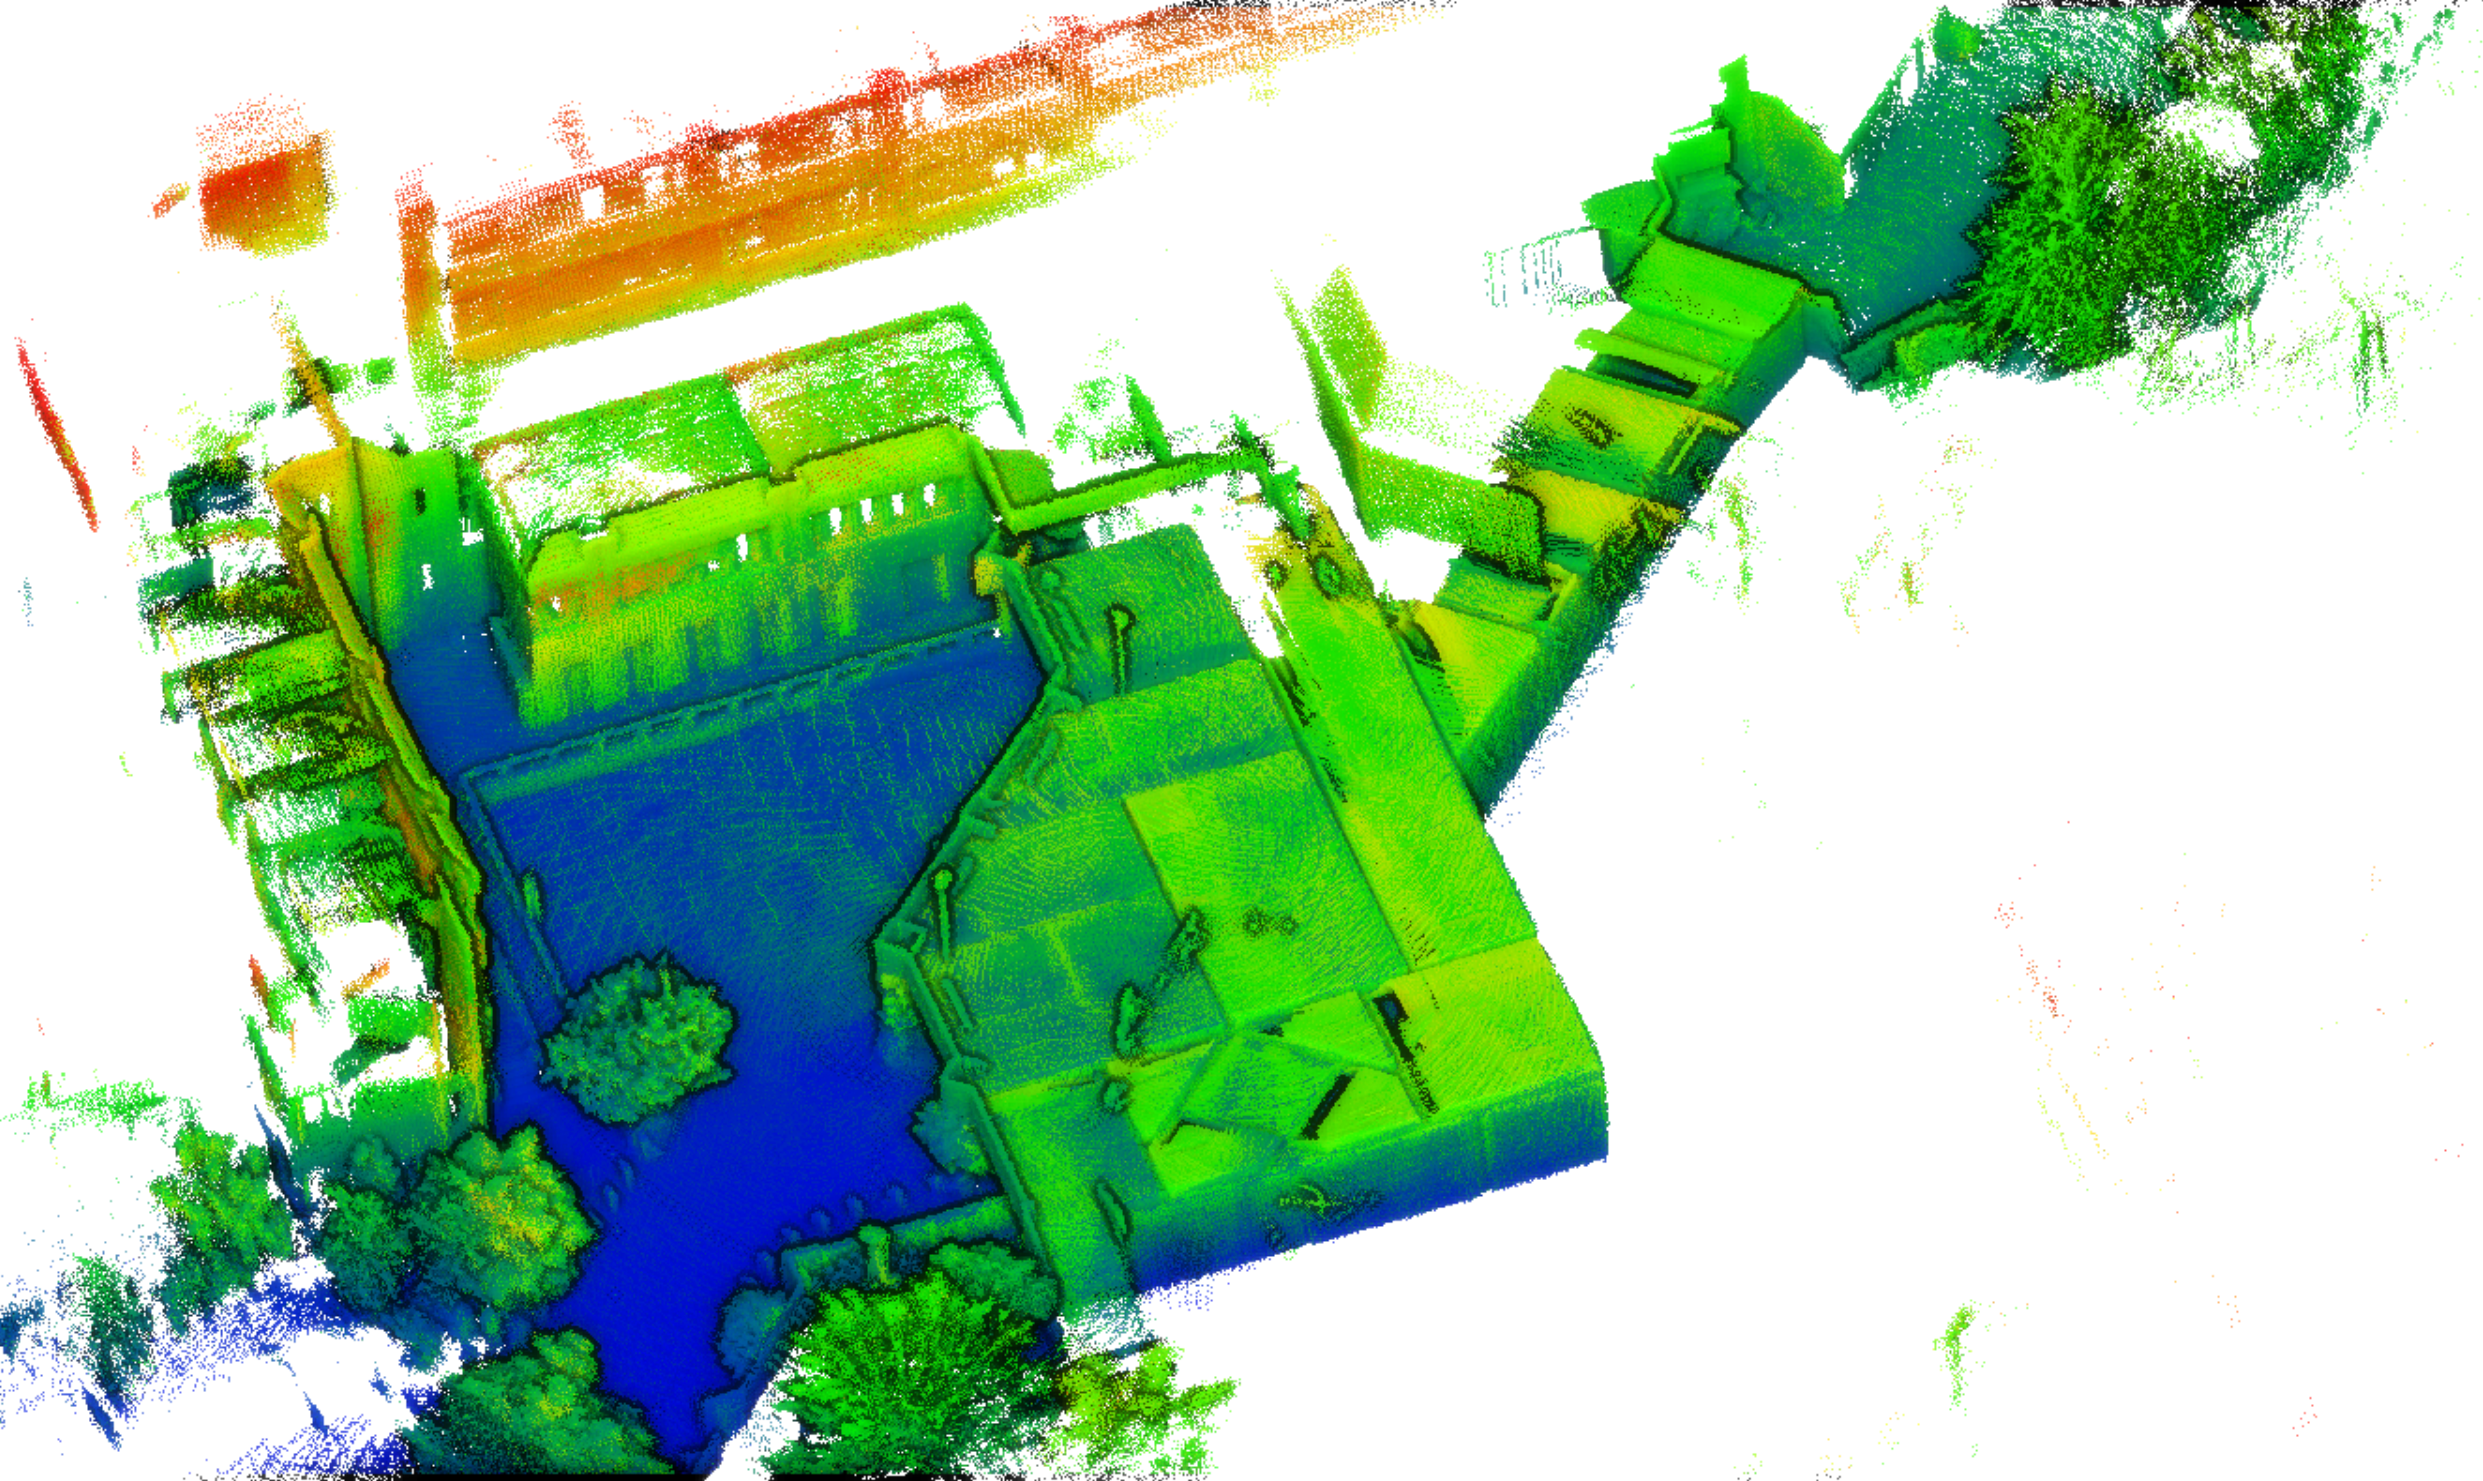
\includegraphics[width=1.0\linewidth]{physik_corrected}
  		\centering \caption{Punktwolke basierend auf der korrigierten Initialschätzung.}
  		\label{fig:physik_corrected}
	\end{subfigure}
	\caption{Wie Abbildung \ref{fig:chemnitz_double_walls} zeigt auch diese Abbildung einen Vergleich der Punktwolken vor und nach Korrektur des in diesem Kapitel vorgestellten Algorithmus. Im linken Teil der Abbildung sind doppelte Objekte und Wände in der Punktwolke gekennzeichnet, die durch einen akkumulativen Fehler im SLAM-Verfahren generiert wurden. Auch hier ist eine signifikante Verbesserung der Trajektorie, erkennbar an der kontinuierlichen Punktwolke, die keine doppelten Wände oder Objekte enthält, zu beobachten.}
	\label{fig:physik_double_walls}
\end{figure}


\begin{figure}
		\centering
		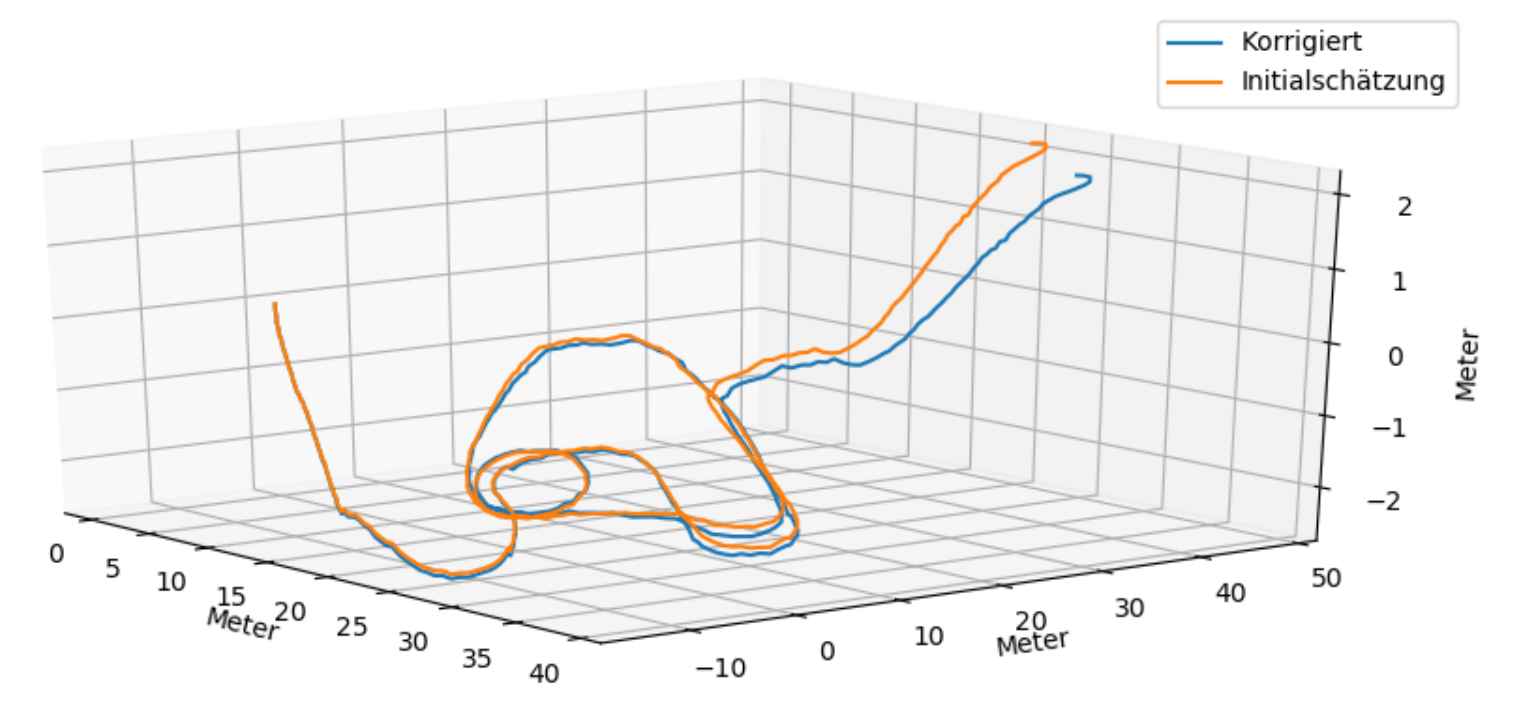
\includegraphics
			[scale=1.0]
			{physik_paths3d}
		\caption
			[Caption for LOF]{Grafische Darstellung der Initialschätzung der Trajektorie im Vergleich mit dem korrigierten Pfad. Es ist eine deutliche Anpassung der Trajektorie zu beobachten. Diese Anpassung sorgt für die in Abbildung \ref{fig:physik_double_walls} erkennbare Kompensation der Fehlerakkumulation und resultiert in einem deutlich besseren Ergebnis, welches keine erkennbaren doppelten Wände ausweist.}                                                                                                                                     
		\label{fig:physik_paths_3d}
\end{figure}


Die in diesem Kapitel entwickelte Lösung wurde hier zunächst vollständig abgekapselt von der TSDF-Karte betrachtet. Dies wird im nachfolgenden Kapitel nun auf Basis der hier vorgestellten Lösung zur Kompensation von akkumulierten Fehler durch die Integration von Schleifenschlüssen und den Ausführungen aus Kapitel \ref{chapter:association} weiter verfolgt.

\section{Kapitel-Zusammenfassung}

In diesem Kapitel wurde die Detektion von Schleifenschlüssen und die darauf aufbauende Optimierung des Pose-Graphen behandelt. Dazu wurde zunächst ein Ansatz zur Detektion der Schleifenschlüsse eruiert und auf das Problem invalider beziehungsweise fehlerhafter Schleifenschlüsse eingegangen. Zur Lösung dieses Problems wurden zwei implementierte Validatoren beziehungsweise Rejector implementiert und vorgestellt. Dadurch können fehlerhafte Schleifenschlüsse identifiziert und verworfen werden. Dies führt zu einem deutlich besseren Ergebnis der Optimierung. Für die Optimierung selbst kommt die Bibliothek GTSAM zum Einsatz. Hier wurde die dazu verwendete Datenstruktur des Faktor-Graphen eingeführt und dessen Funktionsweise, insbesondere über die verwendeten Faktoren, erläutert. Der vorgestellte Ansatz liefert gute Ergebnisse und Vergleiche mit anderen Lösungsansätzen zeigen ähnliche und zum Teil bessere Ergebnisse, wie zu sehen in der Evaluation des Hannover-1 Datensatzes.






